%%%%%%%%%%%%%%%%%%%%%%%%%%%%%%%%%%%%%%%%%%%%%%%%%%%%%%%%%%%%%%%%%%%%%%%%%%%%%%%%
%
% Template license:
% CC BY-NC-SA 3.0 (http://creativecommons.org/licenses/by-nc-sa/3.0/)
%
%%%%%%%%%%%%%%%%%%%%%%%%%%%%%%%%%%%%%%%%%%%%%%%%%%%%%%%%%%%%%%%%%%%%%%%%%%%%%%%%

%----------------------------------------------------------------------------------------
%	PACKAGES AND OTHER DOCUMENT CONFIGURATIONS
%----------------------------------------------------------------------------------------

\documentclass[
11pt, % The default document font size, options: 10pt, 11pt, 12pt
%oneside, % Two side (alternating margins) for binding by default, uncomment to switch to one side
%chapterinoneline,% Have the chapter title next to the number in one single line
spanish,
singlespacing, % Single line spacing, alternatives: onehalfspacing or doublespacing
%draft, % Uncomment to enable draft mode (no pictures, no links, overfull hboxes indicated)
%nolistspacing, % If the document is onehalfspacing or doublespacing, uncomment this to set spacing in lists to single
%liststotoc, % Uncomment to add the list of figures/tables/etc to the table of contents
%toctotoc, % Uncomment to add the main table of contents to the table of contents
parskip, % Uncomment to add space between paragraphs
codirector, % Uncomment to add a codirector to the title page
headsepline, % Uncomment to get a line under the header
]{MastersDoctoralThesis} % The class file specifying the document structure



%----------------------------------------------------------------------------------------
%	INFORMACIÓN DE LA MEMORIA
%----------------------------------------------------------------------------------------

\thesistitle{Llamador Bluetooth con micrófono para sistema de llamado a enfermera} % El títulos de la memoria, se usa en la carátula y se puede usar el cualquier lugar del documento con el comando \ttitle

% Nombre del posgrado, se usa en la carátula y se puede usar el cualquier lugar del documento con el comando \degreename
\posgrado{Carrera de Especialización en Sistemas Embebidos} 
%\posgrado{Carrera de Especialización en Internet de las Cosas} 
%\posgrado{Carrera de Especialización en Intelegencia Artificial}
%\posgrado{Maestría en Sistemas Embebidos} 
%\posgrado{Maestría en Internet de las cosas}

\author{Ing. Raul Alejandro Camacho Dorado} % Tu nombre, se usa en la carátula y se puede usar el cualquier lugar del documento con el comando \authorname

\director{Ing. Sergio Starkloff (SURIX)} % El nombre del director, se usa en la carátula y se puede usar el cualquier lugar del documento con el comando \dirname
\codirector{Mg. Ing. Ericson Joseph Estupiñan Pineda (FIUBA)} % El nombre del codirector si lo hubiera, se usa en la carátula y se puede usar el cualquier lugar del documento con el comando \codirname.  Para activar este campo se debe descomentar la opción "codirector" en el comando \documentclass, línea 23.

\juradoUNO{Ing. Héctor Lacomi (CITEDEF)} % Nombre y pertenencia del un jurado se usa en la carátula y se puede usar el cualquier lugar del documento con el comando \jur1name
\juradoDOS{Mg. Ing Mara Fusco (UTN - FRH)} % Nombre y pertenencia del un jurado se usa en la carátula y se puede usar el cualquier lugar del documento con el comando \jur2name
\juradoTRES{Esp. Ing. Facundo Adrián Lucianna (FIUBA)} % Nombre y pertenencia del un jurado se usa en la carátula y se puede usar el cualquier lugar del documento con el comando \jur3name

\ciudad{Ciudad Autónoma de Buenos Aires}
%\ciudad{ciudad de Mendoza}

\fechaINICIO{marzo de 2020}
\fechaFINAL{Abril de 2021}


\keywords{Sistemas embebidos, FIUBA} % Keywords for your thesis, print it elsewhere with \keywordnames


\begin{document}


\frontmatter % Use roman page numbering style (i, ii, iii, iv...) for the pre-content pages

\pagestyle{plain} % Default to the plain heading style until the thesis style is called for the body content


%----------------------------------------------------------------------------------------
%	RESUMEN - ABSTRACT 
%----------------------------------------------------------------------------------------

\begin{abstract}
\addchaptertocentry{\abstractname} % Add the abstract to the table of contents
%
%The Thesis Abstract is written here (and usually kept to just this page). The page is kept centered vertically so can expand into the blank space above the title too\ldots
\centering

En la presente memoria se describe el desarrollo de un sistema de llamado a la enfermera desarrollado para la empresa SURIX S.R.L., basado en comunicación por Bluetooth, que reemplazará al actual, basado en comunicación cableada. El sistema consiste en un dispositivo llamador, que se conecta con un terminal de sala y puede enviar solicitudes del paciente, así como informar el estado de su batería de alimentación. El terminal de sala debe recibir estos mensajes y reenviarlos a la terminal de enfermería, y si es necesario iniciar una llamada entre el paciente y la enfermera.

Para el desarrollo de esta aplicación se utilizaron conocimientos relacionados a programación de microcontroladores, protocolos de comunicación, sistemas operativos en tiempo real, testing de software y desarrollo de aplicaciones.

\end{abstract}

%----------------------------------------------------------------------------------------
%	CONTENIDO DE LA MEMORIA  - AGRADECIMIENTOS
%----------------------------------------------------------------------------------------

\begin{acknowledgements}
%\addchaptertocentry{\acknowledgementname} % Descomentando esta línea se puede agregar los agradecimientos al índice
\vspace{1.5cm}

A mis papás Marcela y Javier por todo el apoyo durante el desarrollo del trabajo.
  
A mi director y codirector, Sergio y Ericson, por su orientación y apoyo permanente.

A SURIX por la confianza para realizar el trabajo.

\end{acknowledgements}

%----------------------------------------------------------------------------------------
%	LISTA DE CONTENIDOS/FIGURAS/TABLAS
%----------------------------------------------------------------------------------------

\tableofcontents % Prints the main table of contents

\listoffigures % Prints the list of figures

\listoftables % Prints the list of tables


%----------------------------------------------------------------------------------------
%	CONTENIDO DE LA MEMORIA  - DEDICATORIA
%----------------------------------------------------------------------------------------

\dedicatory{\textbf{Dedicado a mis papás Javier y Marcela.}}  % escribir acá si se desea una dedicatoria

%----------------------------------------------------------------------------------------
%	CONTENIDO DE LA MEMORIA  - CAPÍTULOS
%----------------------------------------------------------------------------------------

\mainmatter % Begin numeric (1,2,3...) page numbering

\pagestyle{thesis} % Return the page headers back to the "thesis" style

% Incluir los capítulos como archivos separados desde la carpeta Chapters

% Chapter 1

\chapter{Introducción general} % Main chapter title

\label{Chapter1} % For referencing the chapter elsewhere, use \ref{Chapter1} 

En este capítulo se describe el contexto actual del cual parte el trabajo y el estado del arte de los sistemas de llamado a enfermera. Además se presentan los objetivos, el alcance del trabajo y se expone su justificación

\label{IntroGeneral}

%----------------------------------------------------------------------------------------

% Define some commands to keep the formatting separated from the content 
\newcommand{\keyword}[1]{\textbf{#1}}
\newcommand{\tabhead}[1]{\textbf{#1}}
\newcommand{\code}[1]{\texttt{#1}}
\newcommand{\file}[1]{\texttt{\bfseries#1}}
\newcommand{\option}[1]{\texttt{\itshape#1}}
\newcommand{\grados}{$^{\circ}$}

%----------------------------------------------------------------------------------------

%\section{Introducción}

%----------------------------------------------------------------------------------------
\section{Antecedentes y análisis de contexto}
\label{sec:AntyCont}

SURIX es una empresa argentina fundada en 1998, que se dedica al desarrollo de sistemas de control de acceso basados en tecnología IP. Actualmente ofrece líneas de productos para el hogar y edificios, aplicaciones tecnológicas personalizadas para corporaciones, industrias, hospitales, centros comerciales, autopistas y entes gubernamentales. Estos productos que exporta a más de 14 países para diversas aplicaciones, por lo que tiene oficinas en Israel y México \cite{surix}.

Entre los productos ofertados por SURIX, se destaca el sistema de llamado a enfermera. Este consta de un dispositivo llamador, que se conecta por cable a un terminal de sala, que a su vez se conecta a través de una red con el terminal de enfermería \cite{helpip}.

Desde el dispositivo llamador, el paciente puede encender la luz de lectura o –lo que es más relevante– requerir la atención del personal de servicio a la habitación. En caso de necesitar atención, el terminal de sala iniciará una llamada VoIP con el terminal de enfermería.

El sistema diferencia un llamado para servicio a la habitacion, asistencia en el baño o asistencia en caso de paro cardíaco, y si fue atendido por enfermería remotamente o se está en presencia de la enfermera. También indica cuando concluye el servicio de la enfermera en el cuarto.

Además permite visibilizar la solicitud y tipo de solicitud, por medio de una luminaria ubicada en el pasillo sobre la puerta de la habitación , que se puede configurar para iluminarse de diversos colores o encenderse intermitentemente en función del tipo de solicitud del paciente.

En la terminal de enfermería se dispone de un panel donde se puede visualizar el estado de cada cama, y el terminal de sala actualmente sólo puede conectarse a dos dispositivos llamadores.

En el mercado existen varias soluciones similares a la que se desea desarrollar, entre las que podemos mencionar:

\begin{itemize}
\item MMCALL: sistema que utiliza tecnologías inalámbricas y dispone de pulsadores de llamada colocados en las habitaciones y baños de los pacientes, a través de los cuales solicitan asistencia presionando un botón. La estación de enfermería muestra el número de habitación o cama asignado a ese pulsador de llamada y simultáneamente activa un cronómetro para garantizar una atención oportuna, de manera que si la llamada no es respondida envía un recordatorio tanto a la estación de enfermería como a todos los relojes inalámbricos, con los que cada miembro del personal puede ser equipado, para asegurar que la llamada sea respondida sin importar en qué parte del hospital se encuentren. Todas las llamadas se registran en la estación de enfermería, lo cual permite sacar reportes de desempeño y rendimiento. El alcance de la señal es de 70 a 80 metros, pero se puede extender utilizando amplificadores y repetidores de señal \cite{mmcall}.	

\item Helpnex: sistema modular que utiliza tecnología IP, dispone de pulsadores para cama y baño que permiten que el paciente solicite asistencia presionando un botón, y permite visualizar y atender el requerimiento, pudiendo detallar el motivo o añadir todo tipo de observaciones sobre la solicitud. Todas las alarmas y tareas quedan registradas en una base de datos. Ofrece control sobre personas en general, pudiendo obtener su ubicación en tiempo real, mediante un tag pequeño y compacto, que permite la localización de la persona, a través de radiofrecuencia sobre las principales salidas del centro, con distinción entre cercanía o apertura de una puerta, con visualización de alarmas en el plano en tiempo real. Permite también alarma para pasillo con diferentes códigos de colores, emitiendo indicación sonora y luminosa. Además ofrece la posibilidad de disponer de un puesto de control para la emisión de informes personalizados, permitiendo conocer todo lo ocurrido en el centro de atención medica. \cite{helpnex}.

\item Llamador de enfermería inalámbrico SEI: sistema desarrollado para clínicas, hospitales, geriátricos, hogares de ancianos o casas particulares con personas con movilidad reducida. Dispone de un llamador en cada habitación identificado por un número, cada uno de estos llamadores dispone de tantos pulsadores como camas posea la habitación. Cuando el paciente presiona el pulsador, se reporta inalámbricamente a una central receptora, encendiendo el LED correspondiente a dicha habitación, y una señal sonora advierte del llamado. Mientras existan llamados activos se oirá un “bip” cada 10 segundos alertando a la persona a cargo del llamado pendiente. Si el llamado lleva activo un tiempo mayor a 5 minutos el LED comenzará a parpadear alertando la demora. Para cancelar el llamado la enfermera o persona a cargo debe dirigirse a la habitación correspondiente y presionar el botón “cancelar” del llamador. Mientras el llamado esté activo, en el llamador destellará un LED indicando dicho estado. El alcance de la señal inalámbrica es de 30 a 35 metros que puede extenderse mediante el uso de retransmisores \cite{sei}.

\end{itemize}

En la tabla \ref{tab:sistemasDeLLamadoEnfermera} se resumen las características del sistema de llamado a enfermera de SURIX y de los demás sistemas mencionados.

\begin{table}[h]
	\centering
	\caption[Sistemas de llamado a enfermera]{Tabla comparativa de los sistemas de llamado a enfermera disponibles en el mercado}
	\begin{tabular}{l c c c c}    
		\toprule
		\textbf{Característica} 	 & \textbf{SURIX} & \textbf{MMCALL} & \textbf{Helpnex} & \textbf{SEI}\\
		\midrule
		Dispositivo llamador inalámbrico                                                    &   &   &   & X \\
Central de enfermera inalámbrica                                                    &   & X & X & X \\
\begin{tabular}[c]{@{}l@{}}Aviso de presencia de \\ enfermera por RFID\end{tabular} & X &   & X &   \\
Sistema de localización de pacientes                                                &   &   & X &   \\
Panel de control                                                                    & X & X & X & X \\
Alarma de pasillo configurable                                                      & X & X & X &   \\
Emisión de informes                                                                 & X & X & X &   \\
		\bottomrule
		\hline
	\end{tabular}
	\label{tab:sistemasDeLLamadoEnfermera}
\end{table}

En la figura \ref{fig:sistemasDeLLamadoactuales} se ilustran los distintos equipos llamadores que se han presentado en esta sección.

\begin{figure}[htpb]
	\centering
	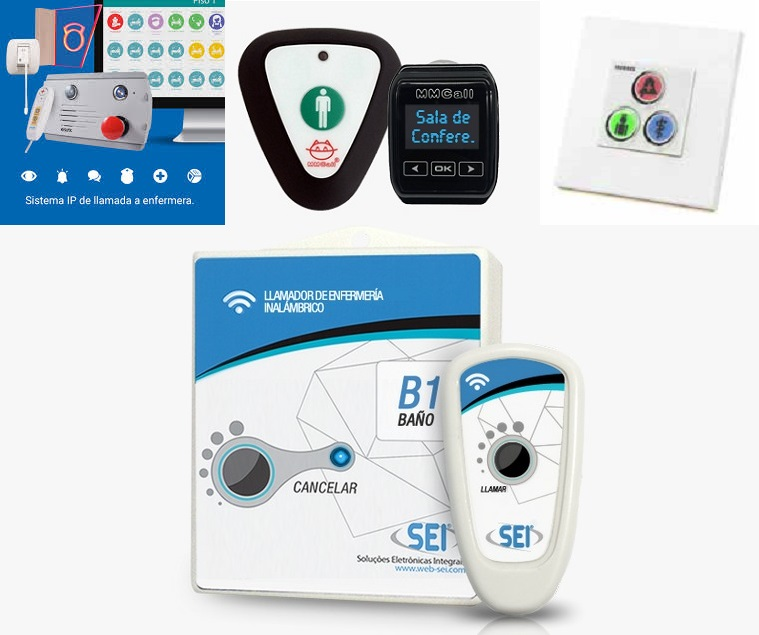
\includegraphics[scale=0.5]{./Figures/llamadores.jpeg}
	\caption{Llamadores de enfermera disponibles en el mercado}
	\label{fig:sistemasDeLLamadoactuales}
\end{figure}


%----------------------------------------------------------------------------------------

\section{Objetivos y Alcance}

\subsection{Objetivos}

El objetivo general de este trabajo es dotar de conectividad Bluetooth al sistema actual de llamado a enfermera de SURIX. Esto permitirá que el sistema de SURIX cuente con un dispositivo llamador inalámbrico, y una central de enfermera inalámbrica. Adicionalmente permitirá en un futuro que se implemente un sistema de localización de pacientes.

Para el logro del objetivo planteado el trabajo contempla:

\begin{itemize}

\item El diseño e implementación de un módulo de expansión que permita dotar de conectividad Bluetooth a la terminal de sala del sistema actual de SURIX.

\item El diseño e implementación de un nuevo dispositivo llamador con conectividad Bluetooth.

\item El desarrollo del firmware para el módulo de expansión diseñado.

\item El desarrollo del firmware para el nuevo dispositivo llamador.

\item El desarrollo del firmware de la terminal de sala para el control de módulo de expansión diseñado.

\end{itemize}

\subsection{Alcance}

El alcance del trabajo está definido por las siguientes consideraciones:

\begin{itemize}
\item Si bien en el trabajo uno de los objetivos es desarrollar el firmware para control del módulo de expansión, esto no implica sustituir el firmware de la terminal de sala por uno nuevo, sino sólo escribir el módulo que permita interactuar a la terminal de sala con el módulo de expansión diseñado, ya que el resto del sistema actual se seguirá utilizando.	

\item Debido a que el diseño del dispositivo llamador debe ser de bajo consumo de energía, este no dispondrá de un parlante, por lo que no se considera el desarrollo de firmware que envíe audio al dispositivo llamador, y la salida de audio se mantendrá en la terminal de sala, como ocurre con el sistema actual.

\item Aunque el diseño del dispositivo llamador implica elegir una fuente de alimentación, el trabajo no contempla diseñar un sistema de recarga para la batería.

\end{itemize}

%----------------------------------------------------------------------------------------

\section{Justificación}

El trabajo permite ampliar la capacidad de conexión de la terminal de sala, que actualmente está limitada a sólo dos dispositivos llamadores, de manera que será posible conectar un mayor número de dispositivos llamadores.

Adicionalmente, los equipos que se conectan mediante cables pueden quedar fuera de servicio cuando el paciente rompe accidentalmente el cable. En cambio, al utilizar conectividad Bluetooth este problema se evita por completo.

Quitar el cable también posibilita que los pacientes que por su estado se encuentren débiles puedan acercar el llamador a su boca haciendo que sea más fácil escuchar su voz.

El hecho de que el dispositivo llamador sea inalámbrico permite que pueda ser utilizado en distintos lugares, lo que permite reorganizar fácilmente una sala, o incluso usar el dispositivo llamador en otra sala, donde sea requerido.

Por otro lado, el dotar de conectividad Bluetooth al sistema actual permitirá a SURIX posicionar este producto para competir con otros sistemas existentes en el mercado, que ya ofrecen esta característica.

\chapter{Introducción específica} % Main chapter title

\label{Chapter2}

%----------------------------------------------------------------------------------------
%	SECTION 1
%----------------------------------------------------------------------------------------
En el presente capítulo se brinda una explicación del funcionamiento general del sistema implementado, y una introducción a diferentes tecnologías utilizadas en el trabajo. Se presentan además los requerimientos y la planificación del trabajo.

\section{Bluetooth}

La tecnología Bluetooth opera en la banda de frecuencia industrial, científica y médica (ISM) sin licencia de 2.4GHz, admite múltiples opciones de radio que permiten a los desarrolladores desarrollar productos que cumplen con requisitos de conectividad únicos en el mercado. 

Ya sea que un producto transmita audio de alta calidad entre un teléfono inteligente y un altavoz, transfiera datos entre una tableta y un dispositivo médico, o envíe mensajes entre miles de nodos en una aplicación de automatización de edificios, los tecnologías Bluetooth Low Energy (LE) y Basic Rate/Enhanced Data Rate (BR/EDR) están diseñadas para satisfacer las necesidades únicas de los desarrolladores de todo el mundo \cite{bluetooth}.


\subsection{Bluetooth low energy (LE)}

La tecnología Bluetooth Low Energy (LE) está diseñada para funcionar con muy baja potencia. Permite un funcionamiento confiable en la banda de frecuencia de 2.4 GHz, aprovecha un sólido enfoque de espectro ensanchado por salto de frecuencia que transmite datos a través de 40 canales \cite{bluetooth}.

Esta tecnología, brinda a los desarrolladores una enorme flexibilidad, incluidas múltiples opciones PHY que admiten velocidades de datos de 125 Kb/s a 2 Mb/s, múltiples niveles de potencia, entre 1 mW y 100 mW, así como múltiples opciones de seguridad \cite{bluetooth}. 

Bluetooth LE también admite múltiples topologías de red, incluidas redes punto a punto, de broadcast y de malla.


\subsection{Bluetooth clásico}

La tecnología Bluetooth clásica, también conocida como Bluetooth Basic Rate/Enhanced Data Rate (BR/EDR), está diseñada para un funcionamiento de baja potencia y también aprovecha un sólido enfoque de salto de frecuencia adaptable, que transmite datos en 79 canales \cite{bluetooth}.

Esta tecnología incluye múltiples opciones PHY que admiten velocidades de datos de 1 Mb/s a 3 Mb/s, múltiples niveles de potencia, entre 1 mW y 100 mW, múltiples opciones de seguridad y una topología de red punto a punto \cite{bluetooth}.

La tabla \ref{tab:Bluetooth} muestra una comparación de las principales características de ambas tecnologías Bluetooth: LE y BR/EDR $\pi$.

\begin{table}[h]
	\centering
	\caption[Tecnologías Bluetooth]{Tabla comparativa de tecnologías Bluetooth}
	\begin{tabular}{l c c}    
		\toprule
		\textbf{} 	 & \textbf{Bluetooth low energy (LE)} & \textbf{Bluetooth clásico}\\
		\midrule
		\begin{tabular}[c]{@{}l@{}}Bandas de \\ frecuencia\end{tabular}          & \begin{tabular}[c]{@{}l@{}}Banda ISM de 2.4GHz \\ (2.402 - 2.480 GHz utilizados)\end{tabular}                                                     & \begin{tabular}[c]{@{}l@{}}Banda ISM de 2.4GHz\\ (2.402 - 2.480 GHz utilizados)\end{tabular}                          \\
Canales                                                                  & \begin{tabular}[c]{@{}l@{}}40 canales con espaciado de 2 \\ MHz (3 canales publicitarios, \\ 37 canales de datos)\end{tabular}                    & \begin{tabular}[c]{@{}l@{}}79 canales con espaciado de \\ 1 MHz\end{tabular}                                          \\
\begin{tabular}[c]{@{}l@{}}Uso de los \\ canales\end{tabular}            & \begin{tabular}[c]{@{}l@{}}Espectro ensanchado por \\ salto de frecuencia (FHSS)\end{tabular}                                                     & \begin{tabular}[c]{@{}l@{}}Espectro ensanchado por \\ salto de frecuencia (FHSS)\end{tabular}                         \\
Modulación                                                               & GFSK                                                                                                                                              & GFSK, $\pi$/4 DQPSK, 8DPSK                                                                                                \\
\begin{tabular}[c]{@{}l@{}}Consumo de\\ energía\end{tabular}             & \begin{tabular}[c]{@{}l@{}}$\sim$0.01x 0.5x de referencia\\ (dependiendo del caso de uso)\end{tabular}                                            & 1 (valor de referencia)                                                                                               \\
\begin{tabular}[c]{@{}l@{}}Velocidad de\\ datos\end{tabular}             & \begin{tabular}[c]{@{}l@{}}LE 2M PHY: 2 Mb/s\\ LE 1M PHY: 1 Mb/s\\ LE Coded PHY (S=2): 500 Kb/s\\ LE Coded PHY (S=8): 125 Kb/s\end{tabular}       & \begin{tabular}[c]{@{}l@{}}EDR PHY (8DPSK): 3 Mb/s\\ EDR PHY ($\pi$/4 DQPSK): 2 Mb/s\\ BR PHY (GFSK): 1 Mb/s\end{tabular} \\
\begin{tabular}[c]{@{}l@{}}Potencia máxima\\ de Transmision\end{tabular} & \begin{tabular}[c]{@{}l@{}}Clase 1: 100 mW (+20 dBm)\\ Clase 1.5: 10 mW (+10 dbm)\\ Clase 2: 2.5 mW (+4 dBm)\\ Clase 3: 1 mW (0 dBm)\end{tabular} & \begin{tabular}[c]{@{}l@{}}Clase 1: 100 mW (+20 dBm)\\ Clase 2: 2.5 mW (+4 dBm)\\ Clase 3: 1 mW (0 dBm)\end{tabular}  \\
\begin{tabular}[c]{@{}l@{}}Topologias\\ de red\end{tabular}              & \begin{tabular}[c]{@{}l@{}}Punto a punto (incluida piconet)\\ Transmisión\\ Malla\end{tabular}                                                    & Punto a punto (incluida piconet)\\
		\bottomrule
		\hline
	\end{tabular}
	\label{tab:Bluetooth}
\end{table}

%----------------------------------------------------------------------------------------

\section{Sistema Propuesto}

La figura \ref{fig:DiagramaBloques} muestra un diagrama de bloques del sistema propuesto donde se puede apreciar que es completamente inalámbrico, ya que el dispositivo llamador se conecta a la terminal de sala a través de bluetooth, esto permitirá eliminar la limitación de ésta para recibir solo dos dispositivos llamadores, además de eliminar los riesgos asociados al cableado, tambien lo hace más cómodo y versátil, pues el paciente podrá llevarlo con él a donde sea que vaya y lo podrá utilizar sin estar necesariamente en la cama, por ejemplo si necesita ir al baño y estando ahí requiere ayuda, no necesita volver a la cama para solicitar atención.

\begin{figure}[htpb]
	\centering
	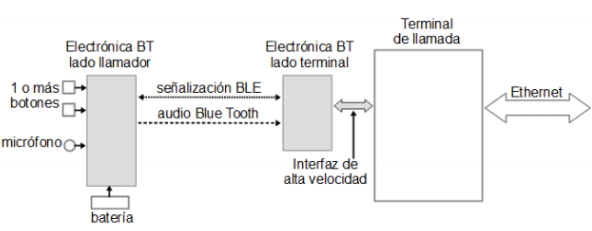
\includegraphics[scale=0.5]{./Figures/DiagramaDeBloques.png}
	\caption{Diagrama en bloques del sistema propuesto}
	\label{fig:DiagramaBloques}
\end{figure}

El sistema desarrollado agrega la electrónica tanto del lado del llamador como del lado de la terminal, cuyo dispositivo bluetooth acepta varios llamadores bluetooth, que le envían novedades. La terminal de sala  a su vez redirecciona las novedades de cada paciente a la terminal de llamada.

La terminal de llamada como ya hacía el anterior sistema notifica vía ethernet a la enfermera, y en caso necesario establece una llamada entre el paciente y la enfermera.

El nuevo sistema cambia la ubicación del micrófono al dispositivo llamador, de manera que ahora esta más cerca del paciente, manteniendo el parlante en la terminal de sala, mejorando así la comunicación.

El microfono seleccionado utiliza la interfaz de audio digital PDM, que es compatible con el procesador elegido dispone de un periférico para controlar micrófonos con este tipo de interfaz.

La comunicación entre el dispositivo Bluetooth y la terminal de llamada se realiza a  través de una interfaz UART, que está disponible en los puertos de accesorios de la terminal de llamada del sistema anterior.

En este sistema el audio se transmite codificado en PCMU, para mantener compatibilidad con el anterior sistema.

%----------------------------------------------------------------------------------------

\section{Requerimientos}

Los requerimientos del nuevo sistema de llamado a enfermera son:

\begin{enumerate}

\item Al pulsar uno de los botones del dispositivo llamador, la terminal de sala deberá iniciar una llamada con una terminal de enfermería.

\item Una vez que la terminal de enfermería conteste a la llamada de la terminal de sala, o cuando la terminal de enfermería realice una solicitud de iniciar una llamada, la terminal de sala indicará al dispositivo llamador, que corresponda, encender su micrófono e iniciar el envío de la señal de audio.

\item Cada dispositivo llamador debe poder identificarse con un ID único de manera que pueda ser registrado en una terminal de sala.

\item La terminal de sala deberá registrar los IDs de los llamadores correspondientes a las camas que tenga en el cuarto, y no deberá aceptar conexiones de otros llamadores.

\item La transmisión de audio debe realizarse por Bluetooth LE.

\item La transmisión de audio debe realizarse utilizando el codec g711 ulaw empleado en el software actual.

\item El dispositivo llamador debe permanecer en modo de bajo consumo mientras no esté en una llamada, o el paciente presione un botón.

\item La terminal de sala además de sus tareas habituales debe estar a la escucha de los mensajes de los dispositivos llamadores que tenga registrados.

\item Al requerimiento de la terminal de enfermería, la terminal de sala debe poder determinar a qué dispositivo llamador dirigir la solicitud.

\item El software debe permitir modificar sus parámetros operativos y almacenarlos en memoria segura.

\item El software no debe alterar las condiciones de operación actuales  del sistema.

\item Se deberá diseñar dos placas eléctricas, una para el modulo de expansión a conectarse a la terminal de sala, y otra para el dispositivo llamador.

\end{enumerate}

Los requerimientos del  modulo de expansión para la terminal son:

\begin{enumerate}

\item Conectar de 1 a 3 dispositivos llamadores.

\item Notificar a la terminal de sala las solicitudes del paciente para que inicie una llamada con la terminal de enfermería.

\item Notificar a la terminal de sala cuando un dispositivo llamador se encuentre con baja batería.

\item Al estar en llamada, el módulo de expansión deberá ignorar las peticiones de otros llamadores y solo retransmitir la señal de audio a la terminal de sala.

\end{enumerate}

Los requerimientos del dispositivo llamador son:

\begin{enumerate}

\item Medir el nivel de batería del dispositivo y notificar al módulo de expansión de la terminal de sala al que se encuentre conectado.

\item Notificar a la terminal de sala sobre las solicitudes del paciente según el botón presionado.

\item Leer señal de audio y transmitirla a la terminal de sala cuando se encuentre en llamada.

\end{enumerate}

\section{Planificación}

En la figura \ref{fig:ActivityOnNode} se presenta la planificación inicial aprobada para el desarrollo del presente proyecto donde se aprecia el camino crítico para su ejecución, habiéndose estimado un total de 615 horas de trabajo.

\begin{figure}[htpb]
	\centering
	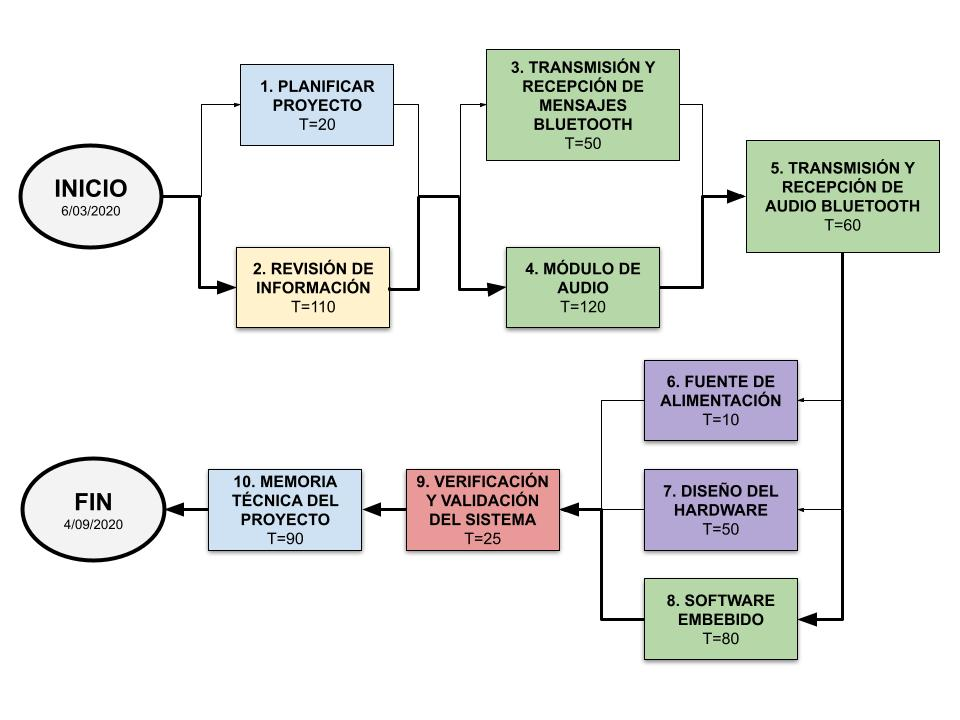
\includegraphics[scale=0.4]{./Figures/ActivityOnNode.jpg}
	\caption{Diagrama activity on node del trabajo}
	\label{fig:ActivityOnNode}
\end{figure}

Sin embargo, esta planificación inicial no se ha podido cumplir debido a que algunos supuestos del proyecto no se cumplieron, entre los que citamos:

\begin{itemize}

\item El tiempo requerido para el desarrollo del software resultó mayor al previsto. Además de ello, se tuvo un retraso en el inicio de esta actividad ya que debido a la cuarentena que se decretó de un momento a otro, no se dispuso oportunamente del material necesario para desarrollar el proyecto.

\item Hubo dificultad al conseguir algunos componentes electrónicos necesarios, particularmente, el micrófono para poder hacer pruebas durante el desarrollo.

\item El tiempo requerido para el desarrollo del hardware resultó mayor al previsto. La empresa cuenta con un fabricante de placas de su confianza, el mismo que se encuentra en la China, motivo por el cual debido a la coyuntura originada en la pandemia por la aparición del COVID-19, que aqueja al planeta, se han tenido dificultades en la comunicación y transporte.

\end{itemize} 
	\chapter{Diseño e implementación} % Main chapter title

\label{Chapter3}

En este capítulo se describe el diseño e implementación de los diferentes módulos de software y hardware del sistema, como así también las diferentes herramientas utilizadas.




%----------------------------------------------------------------------------------------
%	SECTION 1
%----------------------------------------------------------------------------------------
\section{Diseño de hardware}

El sistema propuesto reemplazará al sistema actual de SURIX, el mismo que es un llamador cableado que se conecta en uno de los puertos de accesorio que tiene el terminal de sala, y donde tanto el micrófono como el parlante se encuentra ubicado en dicho terminal.

El nuevo sistema cambia la ubicación del micrófono al dispositivo llamador, de manera que ahora está más cerca del paciente. De esta forma se mantiene el parlante en la terminal de sala, mejorando así la comunicación.

El micrófono seleccionado utiliza la interfaz de audio digital PDM, que es compatible con el procesador elegido dispone de un periférico para controlar micrófonos con este tipo de interfaz.

La comunicación entre el dispositivo Bluetooth y la terminal de llamada se realiza a  través de una interfaz UART, que está disponible en los puertos de accesorios de la terminal de llamada del sistema anterior.
En este sistema el audio se transmite codificado en PCMU, para mantener compatibilidad con el anterior sistema.

Aunque la idea inicial era diseñar dos placas electrónicas distintas: una para el dispositivo llamador y, otra para el lado del terminal sala, que es una placa de extensión de dicho terminal. Luego de realizar los diagramas esquemáticos se vio conveniente diseñar un solo diagrama que sirve para ambos dispositivos. 

Los principales componentes de esta placa son:

\begin{itemize}

\item Un modulo bluetooth LE MDBT42Q-512KV2 que internamente cuenta con un microcontrolador NRF52832 ARM Cortex-M4 de la empresa Nordic, mismo que cumple con las especificaciones de bluetooth LE 5.2, 5.2, 5 y 4.2. Se eligió este módulo porque ya cuenta con una antena de manera que no es necesario diseñar la misma. Este módulo se aprecia en la figura \ref{fig:MDBT42}, y sus principales características se resumen en la tabla \ref{tab:CaracteristicasMDBT42}.

\item Un micrófono digital con interfaz PDM SDM0401-RS261-G04 seleccionado por su bajo costo y tamaño. Este micrófono se puede observar en la figura \ref{fig:mic} y sus características se muestran en la tabla \ref{tab:caracteristicasMic}.

\item El circuito cuenta con la posibilidad de incluir hasta cuatro pulsadores para interacción con el usuario, en el dispositivo llamador. Dicho número puede variar de acuerdo a las versiones de llamador que tiene actualmente la empresa, que varían de 2 a 4 pulsadores según el modelo. También contará con dos LEDs para que el usuario tenga retroalimentación del funcionamiento del dispositivo.

\end{itemize}

\begin{figure}[htpb]
	\centering
	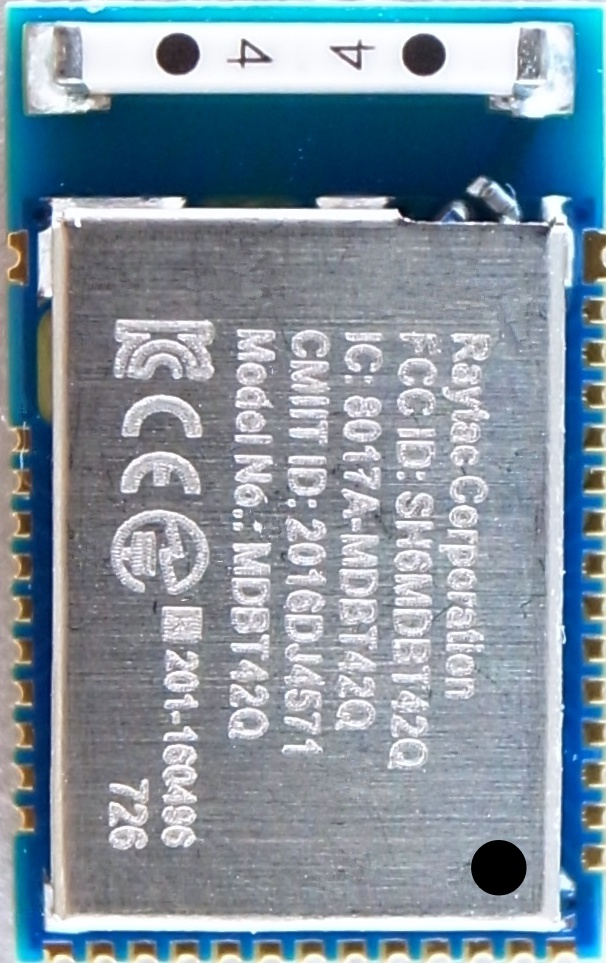
\includegraphics[scale=0.15]{./Figures/MDBT42Q.jpg}
	\caption{Modulo MDBT42Q-512KV2}
	\label{fig:MDBT42}
\end{figure}

\begin{table}[h]
	\centering
	\caption[Características modulo MDBT42Q-512KV2]{Tabla de características modulo MDBT42Q-512KV2}
	\begin{tabular}{l c}    
		\toprule
		\textbf{Característica} 	 & \textbf{Valor}\\
		\midrule
		Tamano (mm)                                                        & 8,8 x 13,8 x 1,8       \\
\begin{tabular}[c]{@{}l@{}}Especificacion\\ Bluetooth\end{tabular} & BT50.1 / BT5.0 / BT4.2 \\
Antena                                                             & Incluida en el modulo  \\
\begin{tabular}[c]{@{}l@{}}Longitud de\\ cobertura\end{tabular}    & \textgreater 80 m      \\
RAM                                                                & 64 Kbytes              \\
Flash                                                              & 512 Kbytes             \\
Pines GPIO                                                         & 32						\\
		\bottomrule
		\hline
	\end{tabular}
	\label{tab:CaracteristicasMDBT42}
\end{table}

\begin{figure}[htpb]
	\centering
	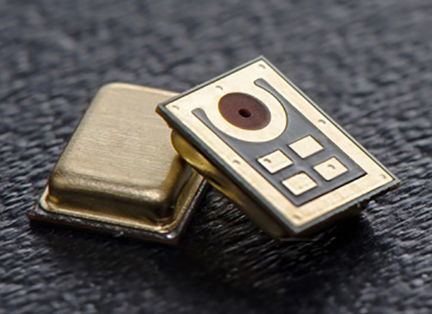
\includegraphics[scale=0.3]{./Figures/mic.png}
	\caption{Micrófono SDM0401-RS261-G04}
	\label{fig:mic}
\end{figure}

\begin{table}[h]
	\centering
	\caption[Características micrófono SDM0401-RS261-G04]{Tabla de características micrófono SDM0401-RS261-G04}
	\begin{tabular}{l c}    
		\toprule
		\textbf{Característica} 	 & \textbf{Valor}\\
		\midrule
		\begin{tabular}[c]{@{}l@{}}Voltaje de\\ alimentacion\end{tabular} & 1.8 V            \\
\begin{tabular}[c]{@{}l@{}}Frecuencia de\\ reloj\end{tabular}     & 2.4 MHz          \\
Directividad                                                      & Omni-Direccional \\
		\bottomrule
		\hline
	\end{tabular}
	\label{tab:caracteristicasMic}
\end{table}

Con estos componentes se diseñó un diagrama esquemático, el cual se muestra en la figura \ref{fig:esquematico}, a partir del cual se fabricó la placa del dispositivo llamador. Esta placa se muestra a en la figura \ref{fig:pcb}.

\begin{figure}[htpb]
	\centering
	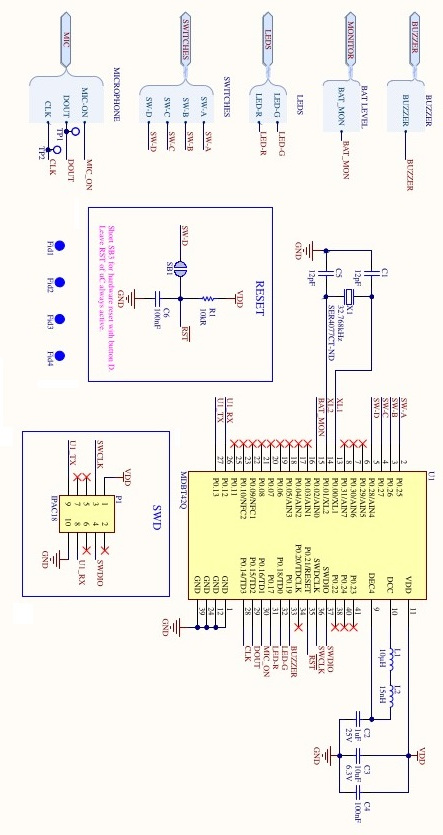
\includegraphics[scale=1]{./Figures/esquematico2.jpeg}
	\caption{Diagrama esquemático para placas Bluetooth}
	\label{fig:esquematico}
\end{figure}


\begin{figure}[htpb]
	\centering
	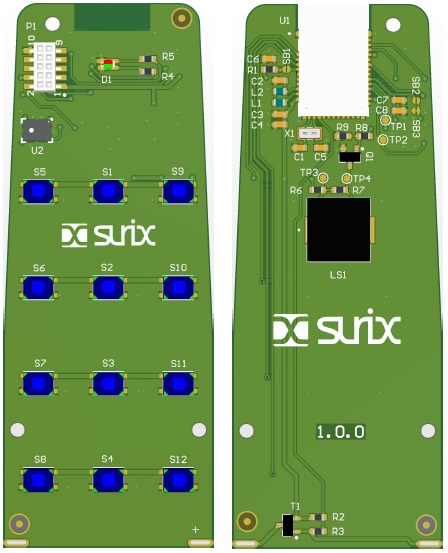
\includegraphics[scale=0.4]{./Figures/placas.jpeg}
	\caption{Placa dispositivo llamador}
	\label{fig:pcb}
\end{figure}

La fabricación de esta placa se ha encargado a una empresa China de confianza de SURIX, y por  motivo de la pandemia de COVID-19 el proceso de envió se retrasó y no es posible mostrarla físicamente.

Para que el circuito pueda ser utilizado tanto en el llamador como del lado de la terminal de llamada se ha previsto que el circuito pueda ser alimentado, por la terminal de sala de SURIX en la terminal de llamada, o por 2 baterías tipo AAA en el dispositivo llamador, estas últimas se escogieron debido principalmente a la facilidad de adquirirlas en el mercado y su relativamente bajo costo.

La placa del dispositivo llamador se aloja dentro de un gabinete plástico, el cual se muestra en la figura \ref{fig:gabinete}, sin embargo este se modificara segun las necesidades de SURIX.

\begin{figure}[htpb]
	\centering
   	\begin{subfigure}[b]{0.3\textwidth}
   		\centering
      	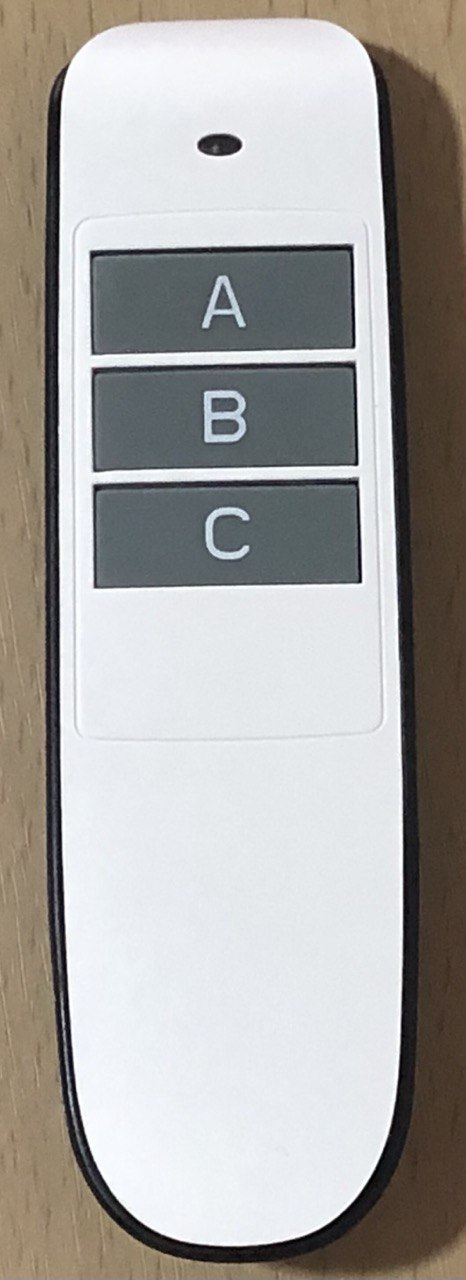
\includegraphics[width=0.6\textwidth]{gabCall.jpeg}
      	\caption{Vista frontal}
   	\end{subfigure}%
   	\begin{subfigure}[b]{0.3\textwidth}
   		\centering
      	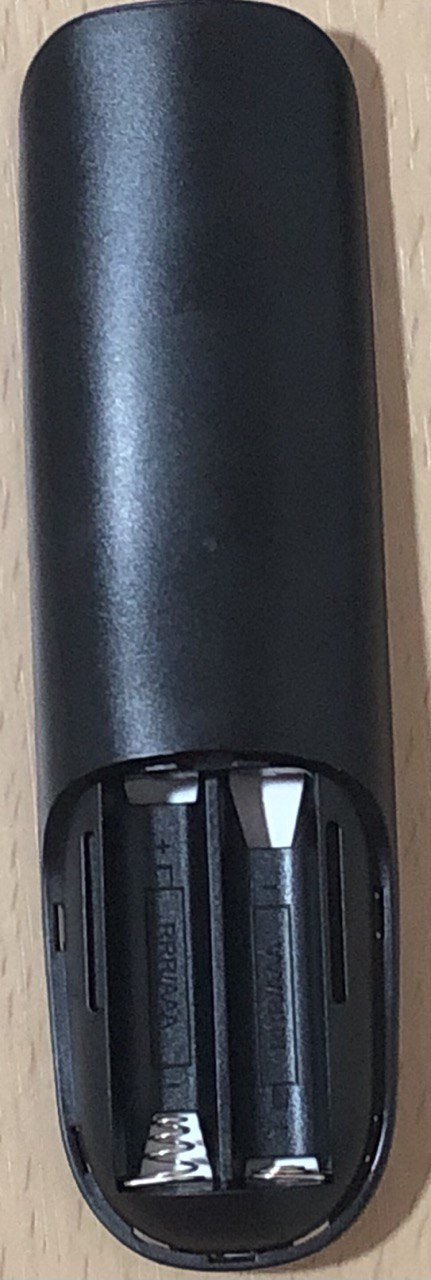
\includegraphics[width=0.6\textwidth]{gabA.jpeg}
      	\caption{Vista trasera con puerto de pilas abierto}
   	\end{subfigure}%
   	\begin{subfigure}[b]{0.3\textwidth}
   		\centering
      	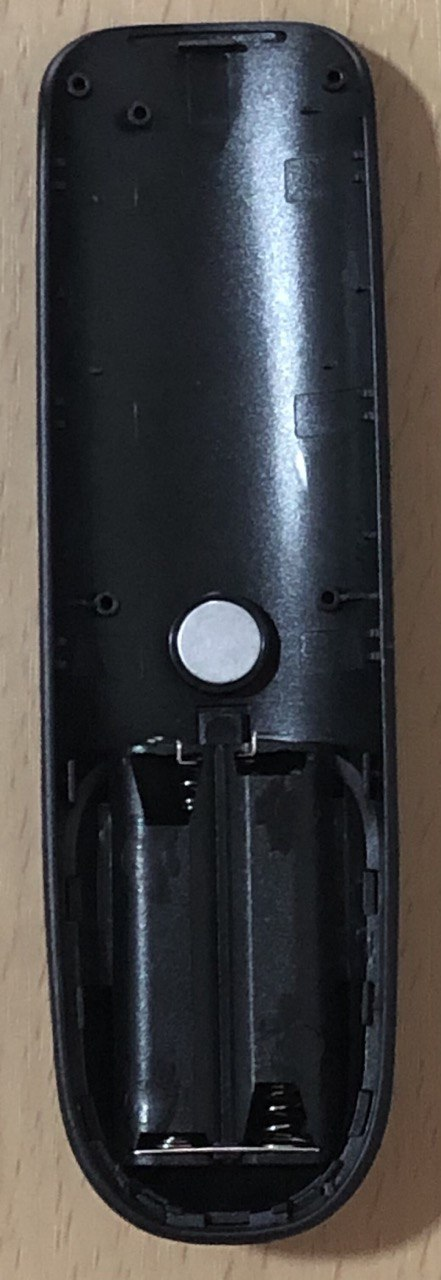
\includegraphics[width=0.6\textwidth]{gabIN.jpeg}
      	\caption{Vista interna}
   	\end{subfigure}%
	\caption{Prototipo gabinete del dispositivo llamador}
	\label{fig:gabinete}
\end{figure}

%----------------------------------------------------------------------------------------
%	SECTION 2
%----------------------------------------------------------------------------------------

\section{Diseño de software}

Para cumplir con los objetivos del trabajo, se dividió el software en tres componentes:

\begin{itemize}

\item El primero que trabaja en bare metal y controla el dispositivo llamador.

\item El segundo también trabaja en bare metal y controla la placa de la terminal de llamada.

\item El tercero es un módulo que se agrega al software del sistema hospitalario de SURIX, el cual trabaja con el sistema operativo FreeRTOS.

\end{itemize}

La implementación de dichos componentes se describen en los apartados \ref{subsec:SoftLlam}, \ref{subsec:SoftCentral} y \ref{subsec:SoftControl}.

\subsection{Software del dispositivo llamador}
\label{subsec:SoftLlam}

En el desarrollo de este firmware se utilizó el paquete de desarrollo de software de Nordic para su familia de microcontroladores 52, de la que es parte el microcontrolador utilizado. Se utilizó la versión 17 de este paquete de desarrollo,  junto con el softdevice s132, que es la implementación más moderna del stack Bluetooth que ofrece esta versión del paquete de desarrollo de Nordic.

Este software se desarrolló utilizando el compilador GCC que proporciona ARM junto con las herramientas de línea de comandos nRF de Nordic.

Para el desarrollo de este firmware se realizó un diagrama statechart UML que describe de manera general el comportamiento de este software. El diagrama mencionado se muestra en la figura \ref{fig:DiagramaSoftLlam}.

\begin{figure}[htpb]
	\centering
	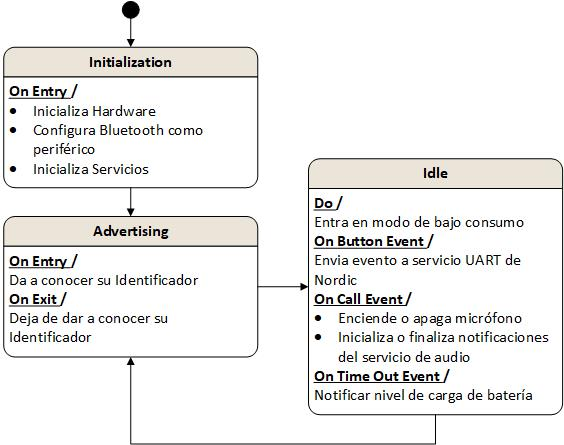
\includegraphics[scale=0.8]{./Figures/DCaller.jpeg}
	\caption{Diagrama de bloques del software del llamador}
	\label{fig:DiagramaSoftLlam}
\end{figure}

Este dispositivo al ser productor de datos en la comunicación Bluetooth, y debido a que sólo se conecta a la central receptora del terminal de sala, se lo programa para que en la conexión cumpla el rol de periférico, definido en el estándar de Bluetooth LE. 

Al estar configurado de esta manera el dispositivo se programó para que inicialmente, entre los datos que lo identifican, envíe el identificador único del microcontrolador durante el proceso de advertising en el cual se da a conocer a todos los dispositivos Bluetooth que están escaneando el ambiente cercano. Dicho identificador usará la central receptora del Bluetooth para decidir a qué dispositivos aceptar una conexión.

Una vez emparejado con una central el dispositivo se mantiene en modo de bajo consumo mientras que el usuario no presione ningún botón en el llamador, o hasta que la central receptora, ubicada en el terminal de sala, le indique que encienda su micrófono para iniciar una llamada con el terminal de enfermería.

Para la notificación de los eventos de presión de botones del dispositivo, el software hace uso de un servicio implementado por la empresa Nordic, Nordic UART Service. Este servicio permite enviar cadenas de caracteres sobre Bluetooth tal como una interfaz serie UART.

Para la parte de audio se implementó un módulo de audio dentro del software, el cual se encarga de inicializar el periférico PDM del microcontrolador para la interacción con el micrófono. Además este módulo se encarga de convertir la señal de 16 khz que entrega el periférico, a una de 8 khz,  para finalmente convertirla a PCMU.

Con la señal de audio en PCMU se requirió implementar un servicio nuevo que permite enviar la señal de voz capturada por el micrófono, ya que no existe uno disponible en el paquete de desarrollo de Nordic. Este servicio está diseñado para que la central receptora le solicite notificar y enviar cada vez que tenga un paquete de 160 muestras de voz. Cuando esto sucede, el dispositivo llamador enciende su micrófono y empieza con el muestreo de voz.

Para cumplir con las especificaciones PCMU, el firmware está configurado para enviar paquetes cada 20 ms, siempre que existan datos para ser transmitidos.

Finalmente el último servicio implementado, en el firmware, es el servicio de notificación de estado de batería, BAS por sus siglas en inglés, que es un servicio estándar en definido por el grupo de interés especial de Bluetooth (Bluetooth SIG). Para poder recolectar los datos que necesita este servicio, se utilizó el conversor analogico digital que lee permanentemente el nivel carga de la batería, el mismo que cada cierto tiempo, configurado para el servicio, notifica a la central receptora.

\subsection{Software de la central receptora}
\label{subsec:SoftCentral}

Para este software se utilizaron las mismas herramientas de desarrollo utilizadas para desarrollar el software del dispositivo llamador, mencionadas en el acápite \ref{subsec:SoftLlam}.

Para el desarrollo de este firmware se realizó un diagrama statechart UML que describe el comportamiento general de este software. El diagrama mencionado se muestra en la figura \ref{fig:DiagramaSoftCentral}.

\begin{figure}[htpb]
	\centering
	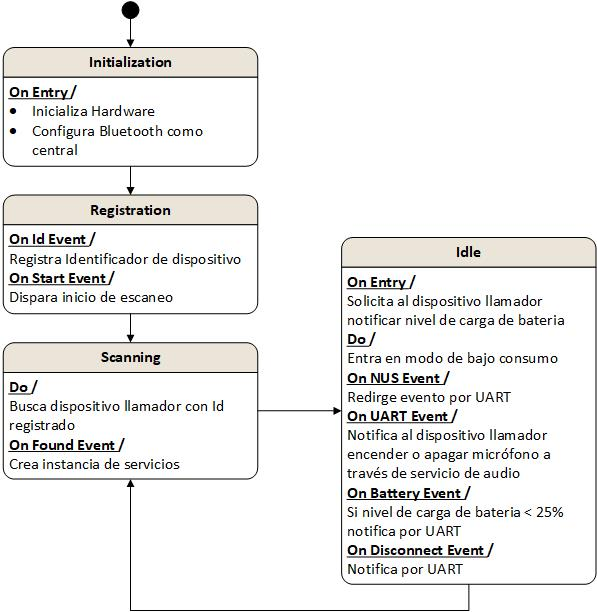
\includegraphics[scale=0.8]{./Figures/Dcentral.jpeg}
	\caption{Diagrama de bloques software central receptora}
	\label{fig:DiagramaSoftCentral}
\end{figure}

Este dispositivo es el encargado de recibir datos de todos los dispositivos llamadores, que tenga conectados. Para ello, este dispositivo se programó para que cumpla el rol de central, dentro del estándar Bluetooth BLE, de manera que este dispositivo es capaz de aceptar conexiones de hasta 7 dispositivos.

Al inicializar este dispositivo, se debe configurar el rol antes mencionado. Sin embargo no empezará a escanear hasta que reciba todos los identificadores de los llamadores a los que aceptara una conexión.

Para recibir estos datos, el dispositivo iniciará la UART presente en el microcontrolador, y esperará a recibir, desde la terminal de sala, las tramas con los identificadores de todos los dispositivos llamadores que tenga asignados para cada cama, los cuales irá guardando en la RAM, en la posición que corresponda según el número de cama recibido, hasta recibir una trama final que le indica que debe empezar a buscar los dispositivos llamadores que tiene registrados. 

Este proceso de búsqueda se mantiene activo hasta que la central logra conectar a todos los dispositivos que tiene asignados. Para descartar los dispositivos no registrados, este proceso lee el identificador que le comparte el dispositivo llamador, verifica que coincida con uno de los identificadores que tiene registrados, y que esté presente el servicio de audio implementado, que también tiene un identificador único. Todo dispositivo que no cumpla con estas dos condiciones será rechazado.

Una vez que un dispositivo logra conectarse, la central receptora creará instancias de los servicios que se mencionan a continuación:

\begin{itemize}

\item Nordic Uart Service (NUS), el cual permite recibir cadenas de caracteres enviadas por los dispositivos llamadores a través de este servicio. A cada mensaje recibido, le agrega el número de cama correspondiente, según el registro de los identificadores, y lo envía al terminal de sala a través de la interfaz UART.

\item Servicio de Audio, que al igual que en el software del dispositivo llamador, se implementó uno nuevo, debido a que no existe uno disponible. Este servicio se encarga de notificar al dispositivo llamador correspondiente, cada vez que se necesita iniciar una llamada, para que este encienda su micrófono y empiece a muestrear, y le solicita notificar, cada vez que tenga una trama de audio en PCMU, la cual recibe a través este servicio. Cuando la central receptora recibe una trama, este servicio se encarga de reenviar dicha trama por la interfaz UART al terminal de sala.

\item Servicio de batería, que como se mencionó en el acápite 3.2.1 es un servicio estándar de Bluetooth LE. Cuando dicho dispositivo se conecta, este servicio le solicitará que empiece a notificar el nivel de carga de su batería. Adicionalmente, la aplicación cada vez que reciba una notificación en este servicio, verifica si está por debajo del 25\%, y de ser así, notifica este evento al terminal de sala, a través de la interfaz UART, identificando al dispositivo llamador en el que se produjo este evento

\end{itemize}

Adicionalmente a estos servicios, la central receptora verifica que todos los dispositivos que tiene conectados, permanezcan conectados. Cuando detecta que un dispositivo no está conectado, envía una notificación al terminal de sala enviando el número de cama al cual el dispositivo llamador estaba registrado.

\subsection{Software de control de la placa de expansión}
\label{subsec:SoftControl}

Este software es un módulo adicional al firmware que SURIX dispone para sus terminales, el mismo que no tiene una sola aplicación, por lo que dependiendo de la aplicación, este módulo se integrará o no al sistema.

El firmware del que forma parte este módulo, es un sistema implementado sobre un sistema operativo FreeRTOS, que ya tiene implementado el protocolo SIP, que permite al módulo realizar llamadas al terminal de enfermería, además de una página web de configuración del terminal.

El comportamiento general de este módulo se observa en el diagrama statechart UML diseñado para su desarrollo, el mismo que se muestra en la figura \ref{fig:DiagramaSoftControl}.

\begin{figure}[htpb]
	\centering
	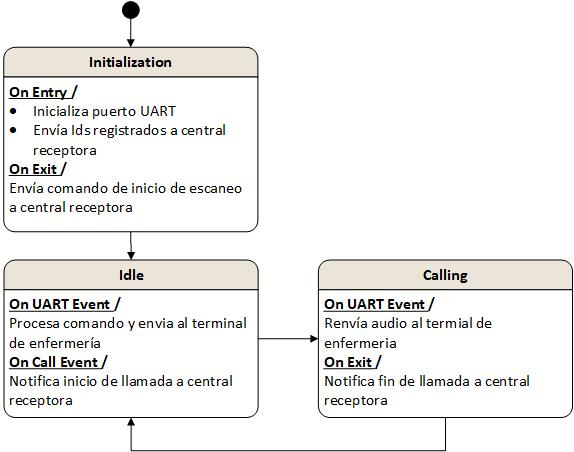
\includegraphics[scale=0.8]{./Figures/Dcontrol.jpeg}
	\caption{Diagrama de bloques software de control de la placa de expansión}
	\label{fig:DiagramaSoftControl}
\end{figure}

Cuando este módulo está presente en el sistema agrega, a la página web del sistema, un menú que le permite al usuario configurar el terminal de sala, para registrar los identificadores de los dispositivos llamadores.

Una vez que el sistema arranca, este módulo lee los identificadores de los dispositivos llamadores ingresados en la web y los envía a la central receptora, y al finalizar esta acción, envía un comando indicando a dicha central que empiece a escanear dichos dispositivos, después de lo cual, se bloquea esperando recibir novedades de esta última.

Cuando este módulo recibe una novedad, identifica el tipo de novedad y la reenvía a través de la red, ya sea local o a través de internet, al terminal de enfermería. Adicionalmente, si la novedad del paciente requiere iniciar una llamada de voz, el módulo notifica al módulo SIP que debe realizar una llamada al terminal de enfermería.

En caso de que una llamada realizada por el terminal de sala es contestada, este módulo se encarga de notificar tal evento a la central receptora para que, esta a su vez, notifique al dispositivo llamador correspondiente.

De la misma manera una vez finalizada la llamada notifica a la central receptora de tal evento para que ésta notifique al dispositivo llamador con el que se estableció la comunicación.

Durante la llamada, este módulo también se encarga de recibir los paquetes de voz de la placa receptora, y mandarlos al buffer RTP para que se transmitan en la llamada SIP.

% Chapter Template

\chapter{Ensayos y resultados} % Main chapter title

\label{Chapter4} % Change X to a consecutive number; for referencing this chapter elsewhere, use \ref{ChapterX}

En este capítulo se presentan las pruebas realizadas para validar el correcto funcionamiento del sistema implementado. Se incluyen pruebas funcionales de cada bloque en particular y de todo el sistema integrado.

%----------------------------------------------------------------------------------------
%	SECTION 1
%----------------------------------------------------------------------------------------

\section{Pruebas funcionales de hardware}
\label{sec:pruebasHW}

Lastimosamente por los retrasos en el inicio  del proyecto, y los problemas con el envío de las placas electrónicas desde China a Argentina debido a la pandemia de COVID-19, no se pudieron realizar ensayos en el hardware final. Sin embargo, se realizó una prueba con la placa de desarrollo en la que se basó el diseño del proyecto. La misma se muestra en la figura \ref{fig:KDRaytac}.

\begin{figure}[htpb]
	\centering
	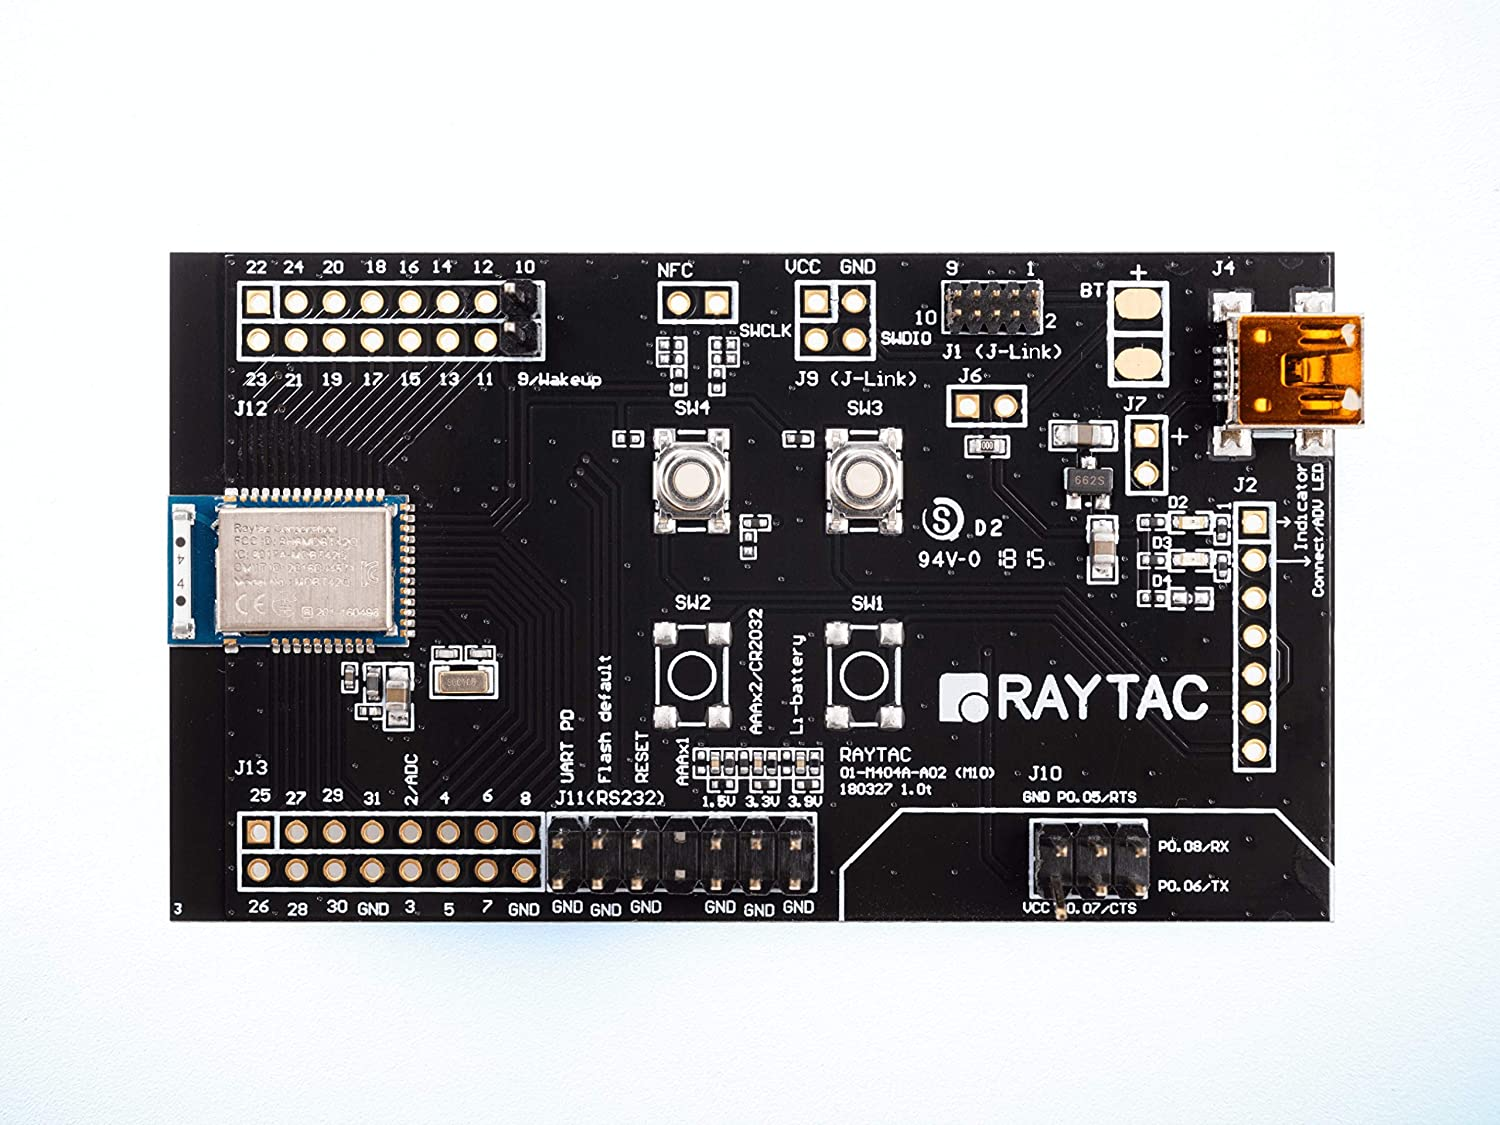
\includegraphics[scale=0.15]{./Figures/DKMDBT42Q-512KV2.jpg}
	\caption{Kit de desarrollo Raytac MDBT42Q-512KV2}
	\label{fig:KDRaytac}
\end{figure}

La prueba se realizó para que SURIX pueda decidir cómo sería la fabricación final de la placa de la central receptora, ya que esta debe estar alojada en los gabinetes en los que la empresa entrega sus productos actualmente, algunos de los cuales tienen una tapa frontal metálica. Esta prueba estaba dirigida a determinar, si el producto final del trabajo, podría ser utilizado en dichos gabinetes sin tener grandes pérdidas de potencia en la señal recibida, En ella, se realizaron mediciones de potencia de señal, tanto con el dispositivo Bluetooth dentro del gabinete metálico, como por fuera de él, para determinar las diferencias.

El gabinete utilizado para esta prueba se puede apreciar en la figura \ref{fig:GMetalico}.

\begin{figure}[htpb]
	\centering
	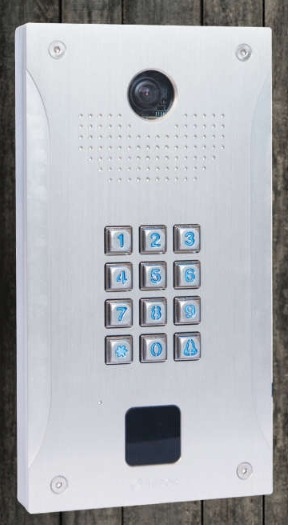
\includegraphics[scale=0.4]{./Figures/gabMet.jpeg}
	\caption{Gabinete metálico SURIX}
	\label{fig:GMetalico}
\end{figure}

Para medir la potencia de la señal se utilizó la aplicación móvil que proporciona Nordic semiconductor, nRFConnect, la cual permite escanear todos los dispositivos Bluetooth que se encuentran dentro del rango de detección del teléfono móvil y muestra la potencia de la señal que recibe de cada uno de ellos.

Los resultados obtenidos se muestran en la figura \ref{fig:Psenal}.

\begin{figure}[!h]
	\centering
   	\begin{subfigure}[b]{0.45\textwidth}
   		\centering
      	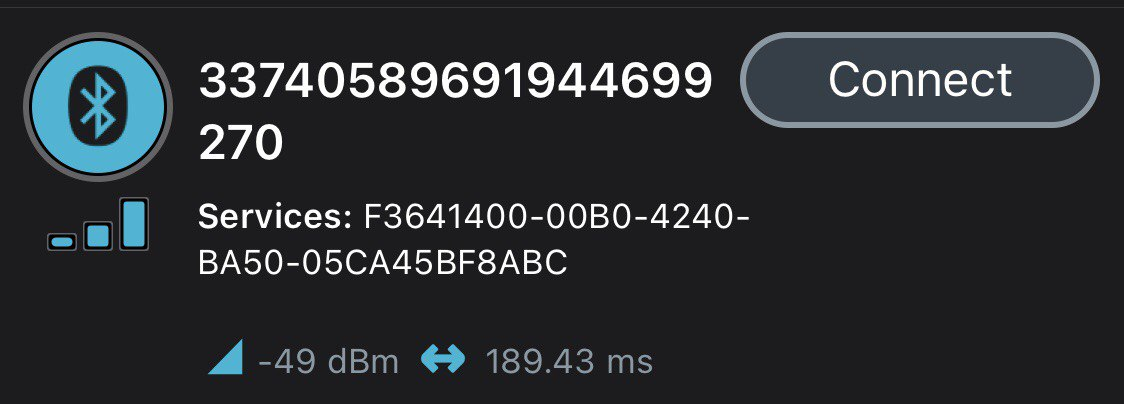
\includegraphics[width=1\textwidth]{signalCO.jpeg}
      	\caption{Medicion a 10 cm de distancia fuera del gabinete}
      	\label{fig:PsenalA}
   	\end{subfigure}%
   	\hfill
   	\begin{subfigure}[b]{0.45\textwidth}
   		\centering
      	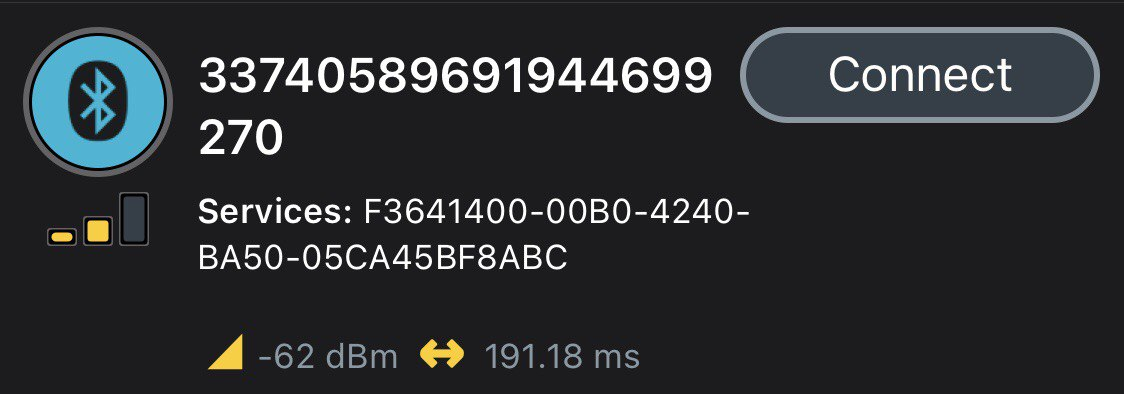
\includegraphics[width=1.03\textwidth]{signalCI.jpeg}
      	\caption{Medicion a 10 cm de distancia dentro del gabinete}
      	\label{fig:PsenalB}
   	\end{subfigure}%
   	\newline
   	\begin{subfigure}[b]{0.45\textwidth}
   		\centering
      	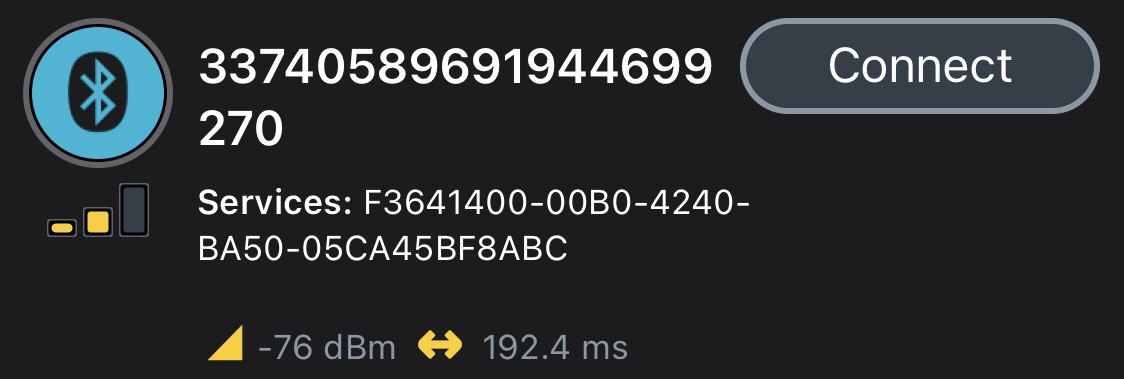
\includegraphics[width=1.04\textwidth]{signalAO.jpeg}
      	\caption{Medicion a 10 m de distancia fuera del gabinete}
      	\label{fig:PsenalC}
   	\end{subfigure}%
   	\hfill
   	\begin{subfigure}[b]{0.45\textwidth}
   		\centering
      	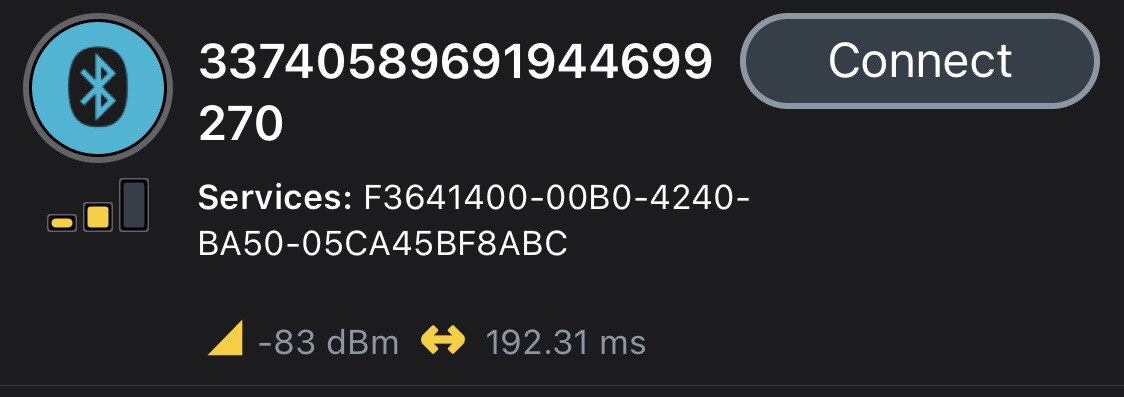
\includegraphics[width=1\textwidth]{signalAI.jpeg}
      	\caption{Medicion a 10 m de distancia dentro del gabinete}
      	\label{fig:PsenalD}
   	\end{subfigure}%
	\caption{Resultados medición potencia de señal recibida del módulo de Bluetooth}
	\label{fig:Psenal}
\end{figure}

En los apartados \ref{fig:PsenalA} y \ref{fig:PsenalB} de la figura se observan las mediciones a 10 cm de distancia del dispositivo Bluetooth dentro y fuera del gabinete metálico respectivamente, existiendo una pérdida de 13 dBm. Y en los apartados \ref{fig:PsenalC} y \ref{fig:PsenalD} se ven las mediciones realizadas a 10 metros de distancia del dispositivo, donde se aprecia una pérdida de tan sólo 7 dBm, por lo que se concluye que las pérdidas son pequeñas y no afectarán a la comunicación.

Finalmente, para determinar de forma práctica que el dispositivo se podría utilizar con estos gabinetes metálicos, se hizo un último ensayo estableciendo una llamada tal como ocurriría  en condiciones reales de uso al interior de una sala de hospital.

Para esto se instaló una placa Bluetooth dentro del gabinete de la figura \ref{fig:GMetalico}, y se la conecto al terminal de sala, que a su vez se conectó a una red local para poder establecer una llamada con un ordenador, en el cual se dispone de softphone (software que permite establecer llamadas VoIP en un ordenador). Por otro lado se usó otro dispositivo Bluetooth con el micrófono conectado y se estableció una llamada con el ordenador.

Los resultados de este ensayo fueron positivos, ya que no se presentaron dificultades durante la llamada, y se escuchó claramente la voz recibida por Bluetooth.

\section{Pruebas unitarias}
\label{sec:pruebasUN}

Las pruebas unitarias se realizaron para cada módulo, conforme se fueron desarrollando, empezando por los más básicos y aquellos que servirían de base para otros.
Para la comunicación Bluetooth, en todos los servicios implementados para el funcionamiento del sistema, cada servicio se implementó y probó, siempre primero del lado del dispositivo llamador, ya que este cumple el rol de periférico, para luego implementar y probar del lado de la central receptora.

Para validar los resultados obtenidos en la central receptora, se hizo uso de la UART del dispositivo, y se reenvió todo lo que se recibía de los servicios por esta interfaz. Para comprobar la correcta recepción de los datos, se conectó el módulo de Bluetooth con el que se realizaron las pruebas, a un adaptador de TTL a USB que permite ver los resultados en el ordenador usando el software cutecom, que no es más que un terminal serial para la PC.

El primer servicio que se probó fue el servicio UART de Nordic, que si bien es un servicio incluido en el paquete de desarrollo de Nordic se decidió hacer la prueba para comprobar que la implementación fue correcta en el firmware. 

Los resultados del lado del llamador se probaron haciendo uso de las aplicaciones de Nordic para móvil: nRFconnect y nRF Toolbox, con la primera se verificó que el servicio ya estaba presente, y con la segunda que al presionar un botón el dispositivo llamador efectivamente enviaba el mensaje programado. Los resultados de esta prueba se muestran en la figura \ref{fig:Pnus}.

\begin{figure}[htpb]
	\centering
   	\begin{subfigure}[b]{0.5\textwidth}
   		\centering
      	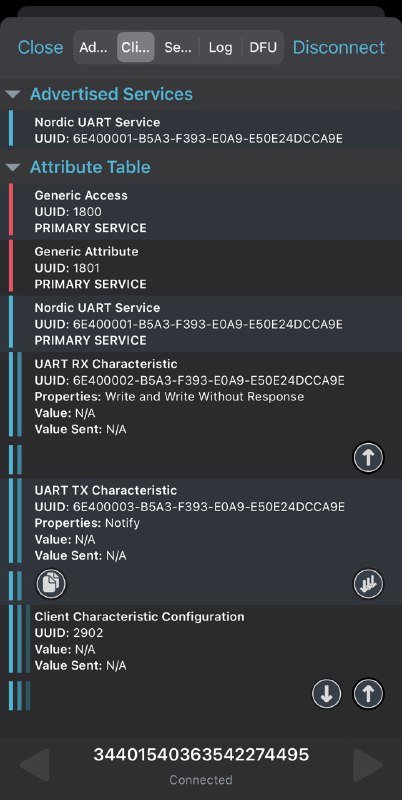
\includegraphics[width=0.8\textwidth]{nusCC.jpeg}
      	\caption{Servicio reconocido en nRFConnect}
      	\label{fig:PnusA}
   	\end{subfigure}%
   	\begin{subfigure}[b]{0.5\textwidth}
   		\centering
      	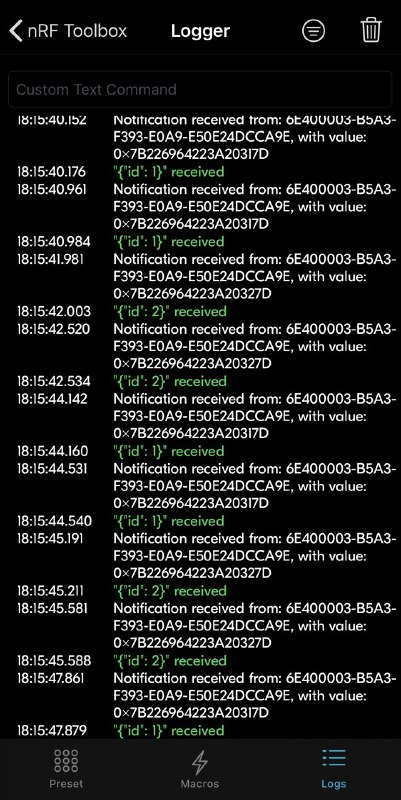
\includegraphics[width=0.8\textwidth]{nusCT.jpeg}
      	\caption{Mensajes recibidos en nRF Toolbox}
      	\label{fig:PnusB}
   	\end{subfigure}%
	\caption{Resultados prueba servicio NUS en el dispositivo llamador}
	\label{fig:Pnus}
\end{figure}

Una vez probado el servicio UART de Nordic en el dispositivo llamador, se probó que también funcionara en la central receptora. Se probó con dos llamadores conectados, para verificar que podía aceptar la conexión de varios periféricos, y que recibía los mensajes de este servicio. Los resultados de esta prueba se muestran en la figura \ref{fig:Pnus2}.

\begin{figure}[htpb]
	\centering
	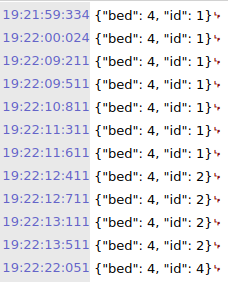
\includegraphics[scale=0.7]{./Figures/Pnus2.png}
	\caption{Resultados prueba servicio de NUS en la central receptora}
	\label{fig:Pnus2}
\end{figure}

El siguiente servicio probado  fue el servicio de audio, pero estas pruebas se exponen en el apartado \ref{sec:pruebasACS} debido a que se implementó desde cero y es el servicio más importante del sistema.

Posteriormente se probó el servicio de batería, que es el encargado de notificar el nivel de carga de batería del dispositivo llamador. Este servicio, al igual que el NUS, viene ya implementado en el paquete de desarrollo de Nordic.

Para probarlo se hizo uso de las dos aplicaciones móviles antes mencionadas, otra vez verificando que el servicio sea reconocido, y que el valor de carga de la batería pueda ser leído. Los resultados de esta prueba se muestran en la figura \ref{fig:Pbas}.

\begin{figure}[htpb]
	\centering
   	\begin{subfigure}[b]{1\textwidth}
   		\centering
      	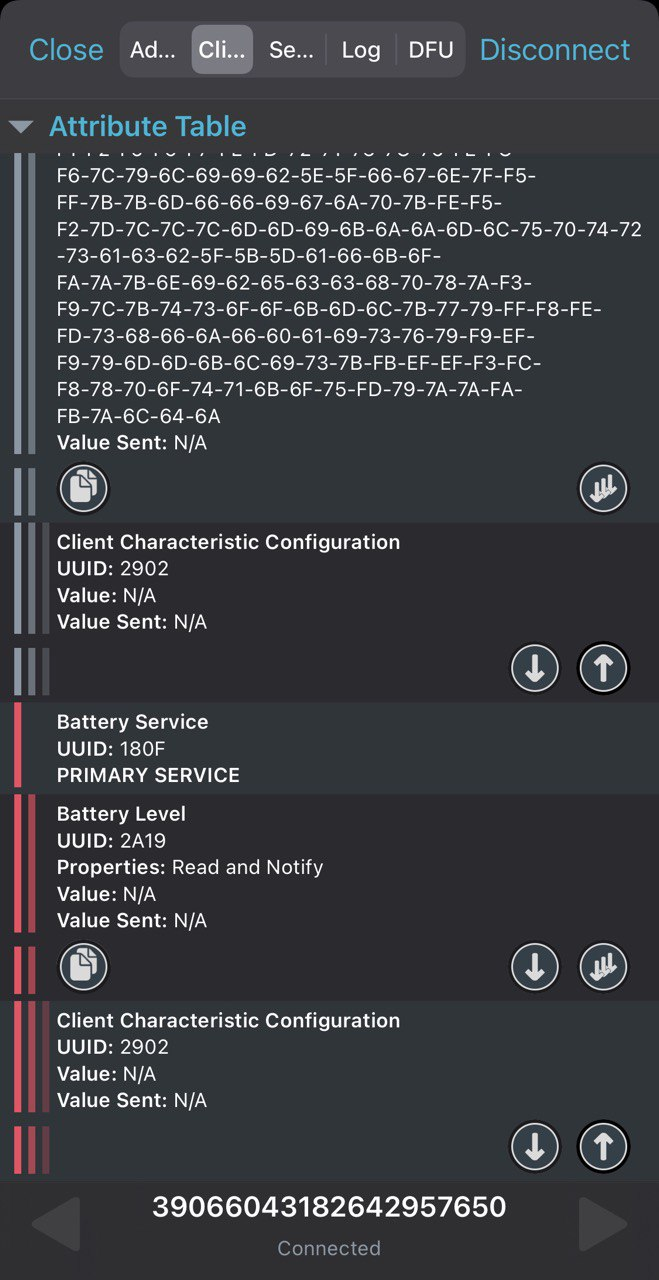
\includegraphics[width=0.5\textwidth]{basCC.jpeg}
      	\caption{Servicio reconocido en nRFConnect}
      	\label{fig:PbasA}
   	\end{subfigure}%
   	\newline
   	\begin{subfigure}[b]{1\textwidth}
   		\centering
      	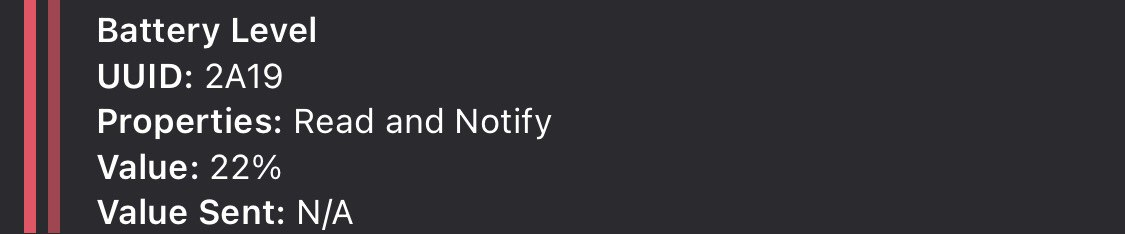
\includegraphics[width=0.7\textwidth]{basCT.jpeg}
      	\caption{Mensajes recibidos en nRF Toolbox}
      	\label{fig:PbasB}
   	\end{subfigure}%
	\caption{Resultados servicio de batería en el dispositivo llamador}
	\label{fig:Pbas}
\end{figure}

Para terminar con la parte bluetooth se probó el servicio de batería en la central receptora, verificando que recibía los niveles de batería y que los notificara por UART si el nivel de batería estaba por debajo del 25\%. Los resultados de esta prueba se muestran en la figura \ref{fig:Pbas2}, y se pueden verificar la notificación con un mensaje con id 3.

\begin{figure}[htpb]
	\centering
	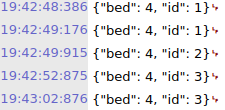
\includegraphics[scale=0.7]{./Figures/Pbas2.png}	
	\caption{Resultados servicio de batería en la central receptora}
	\label{fig:Pbas2}
\end{figure}

Con los servicios de bluetooth probados, se procedió a implementar y probar el módulo de control de la placa expansora. Lo primero que se probó fue que en la web se incluyan los campos para registrar los identificadores de los dispositivos llamadores, y que teniendo registrado algún valor se manden los identificadores por la UART del terminal. Los resultados se muestran en la figura \ref{fig:Pllam}.

\begin{figure}[htpb]
	\centering
   	\begin{subfigure}[b]{1\textwidth}
   		\centering
      	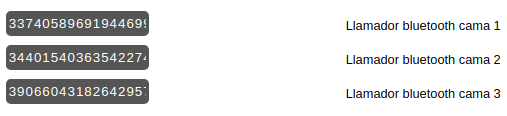
\includegraphics[width=0.8\textwidth]{regcall.png}
      	\caption{Llamadores registrados en pagina web de la terminal de sala}
      	\label{fig:PllamA}
   	\end{subfigure}%
   	\newline
   	\begin{subfigure}[b]{1\textwidth}
   		\centering
      	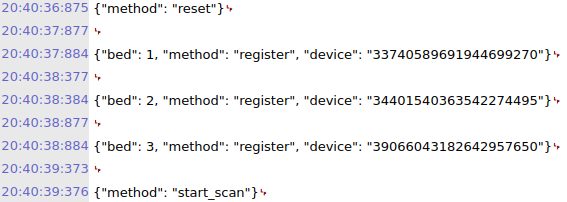
\includegraphics[width=0.8\textwidth]{regcall1.png}
      	\caption{Mensajes enviados para registrar llamadores en central receptora}
      	\label{fig:PllamB}
   	\end{subfigure}%
	\caption{Resultados del registro de identificadores de los dispositivos llamadores}
	\label{fig:Pllam}
\end{figure}

\section{Pruebas de envío y recepción de audio por Bluetooth}
\label{sec:pruebasACS}

Para el envío y recepción de audio, no se tenía ningún servicio disponible en el paquete de desarrollo de Nordic, razón por la cual se implementó desde cero y se realizaron pruebas según se fue implementando. 

Para empezar se desarrolló un driver para controlar el micrófono con la interfaz PDM. Para verificar el funcionamiento de esta interfaz, se utilizó un analizador lógico que permitió ver las señales de reloj y de datos que se recibían del micrófono. Los resultados obtenidos se muestran en la figura \ref{fig:Ppdm}.

\begin{figure}[htpb]
	\centering
	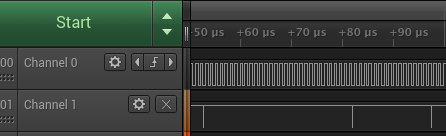
\includegraphics[scale=0.8]{./Figures/pdm.png}	
	\caption{Resultados driver de microfono PDM}
	\label{fig:Ppdm}
\end{figure}

Con la interfaz funcionando, la siguiente tarea fue probar que el servicio implementado en el dispositivo llamador fuera reconocido en la aplicación nRFconnect. Una vez verificado que  el servicio era reconocido, se comprobó que al activar la notificación del servicio los datos del micrófono se puedan ver en la misma aplicación. Los resultados se muestran en la figura \ref{fig:Pacs}.

\begin{figure}[htpb]
	\centering
	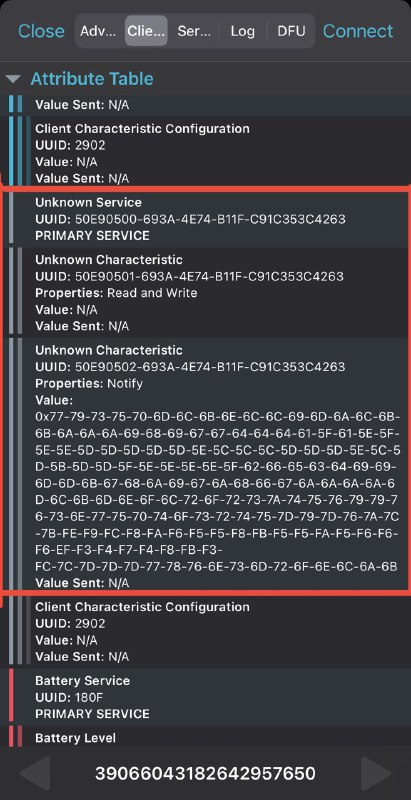
\includegraphics[scale=0.5]{./Figures/acsCC.jpeg}	
	\caption{Resultados servicio de audio en el dispositivo llamador}
	\label{fig:Pacs}
\end{figure}

Del lado de la central receptora se probó que los datos se reciben en el nuevo servicio, y que se pasan directamente a través de UART. La primera prueba de este servicio, fue que los datos del micrófono se pudieran ver en el software cutecom mencionado en el apartado 4.2. Los resultados se muestran en la figura \ref{fig:Pacs2}.

\begin{figure}[htpb]
	\centering
	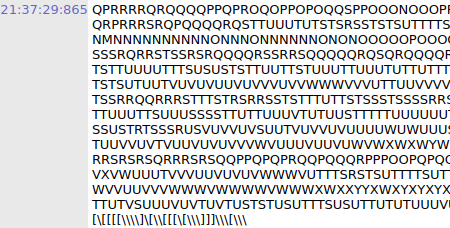
\includegraphics[scale=0.5]{./Figures/acsCR.png}	
	\caption{Resultados servicio de audio en central receptora}
	\label{fig:Pacs2}
\end{figure}

La segunda prueba realizada con los datos recibidos por UART, fue graficar en tiempo real los datos del micrófono, para ello se desarrolló un software en Python. Esta prueba se realizó para comprobar que la onda generada por los datos recibidos, cambiaba en función a los estímulos que recibía el micrófono. Los resultados fueron positivos y se muestran en la figura \ref{fig:Psau}.

\begin{figure}[htpb]
	\centering
	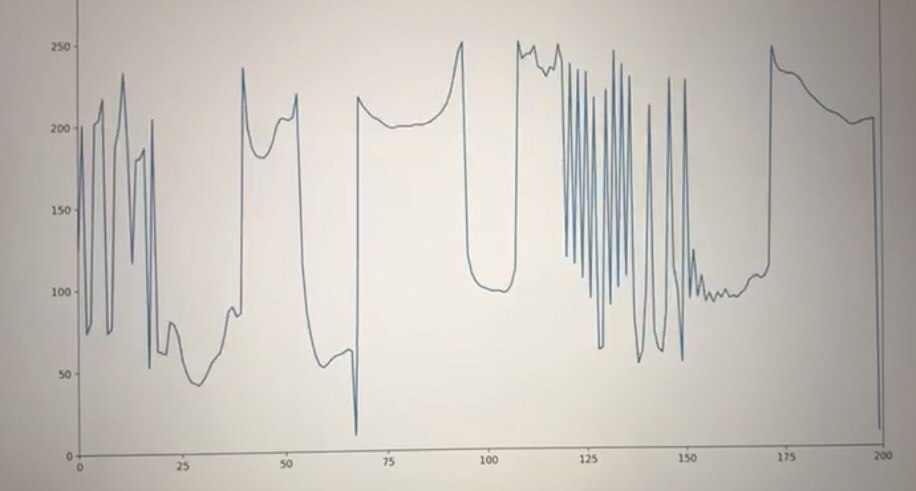
\includegraphics[scale=0.4]{./Figures/callpython.jpeg}	
	\caption{Grafica señal de audio recibida del dispositivo llamador}
	\label{fig:Psau}
\end{figure}

Finalmente, se hizo que los datos del micrófono se envíen al terminal de sala y, que éste los envíe directamente al parlante que tiene conectado. Los resultados finales fueron satisfactorios.

\section{Pruebas de integración}
\label{sec:pruebasInt}

La última etapa de prueba del proyecto fue probar el funcionamiento de todo el sistema en su conjunto. Para verificar esto se registraron dos identificadores correspondientes a dos dispositivos llamadores, que para las pruebas fueron los módulos de desarrollo con los que se trabajó el proyecto.

Para comprobar que los dispositivos llamadores fueron correctamente registrados, después de tener inicializada la central receptora, se comprobó que los llamadores efectivamente se conectaron a la misma, verificando que estuviera encendido el LED indicador de conexión. A continuación, en la figura \ref{fig:Pmcon} se evidencia el estado de conexión de los dispositivos llamadores.

\begin{figure}[htpb]
	\centering
	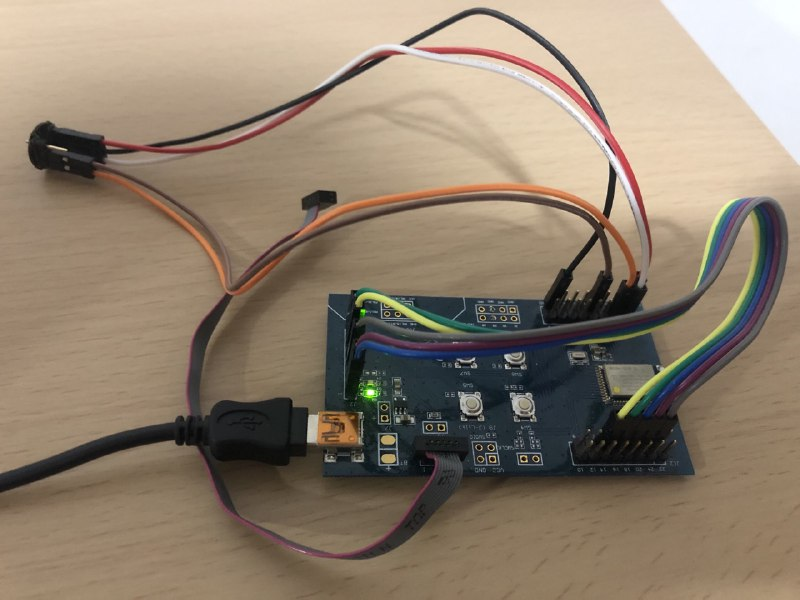
\includegraphics[scale=0.45]{./Figures/callcon.jpeg}	
	\caption{Dispositivo llamador conectado}
	\label{fig:Pmcon}
\end{figure}

Posteriormente, con un analizador lógico conectado en paralelo a la interfaz UART del terminal de sala, se probó que al presionar un botón de uno de los dispositivos llamadores la central receptora reaccionara notificando del evento indicando el número de cama al que está registrado el llamador que originó la novedad. En la figura \ref{fig:Pmrcv} se muestra el resultado de esta prueba.

\begin{figure}[htpb]
	\centering
   	\begin{subfigure}[b]{1\textwidth}
   		\centering
      	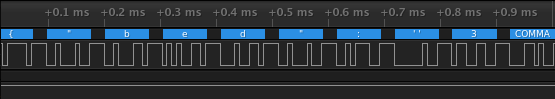
\includegraphics[width=1\textwidth]{intRcv.png}
      	\caption{Mensaje recibido en el terminal de sala}
      	\label{fig:PmrcvA}
   	\end{subfigure}%
   	\newline
   	\begin{subfigure}[b]{1\textwidth}
   		\centering
      	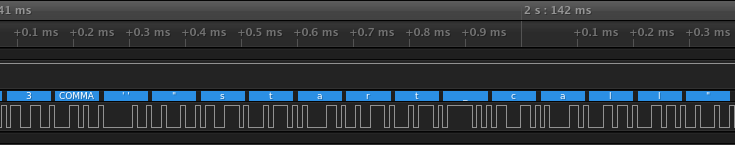
\includegraphics[width=1\textwidth]{intSend.png}
      	\caption{mensaje envido por el terminal de sala al dispositivo llamador}
      	\label{fig:PmrcvB}
   	\end{subfigure}%
   	\newline
   	\begin{subfigure}[b]{1\textwidth}
   		\centering
      	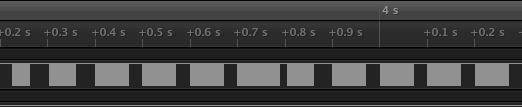
\includegraphics[width=1\textwidth]{intAu.png}
      	\caption{Señal de audio recibida por el terminal de sala}
      	\label{fig:PmrcvC}
   	\end{subfigure}%
	\caption{Mensajes recibidos por el terminal de sala}
	\label{fig:Pmrcv}
\end{figure}

Finalmente la última prueba realizada al sistema fue iniciar una llamada con uno de los llamadores. En la figura \ref{fig:Pmicon} se evidencia un segundo led encendido indicando que el llamador tiene encendido su micrófono, y en la figura \ref{fig:Psrtp} se observa la imagen de una captura de paquetes de la señal de audio que viaja por RTP durante la llamada.

\begin{figure}[htpb]
	\centering
	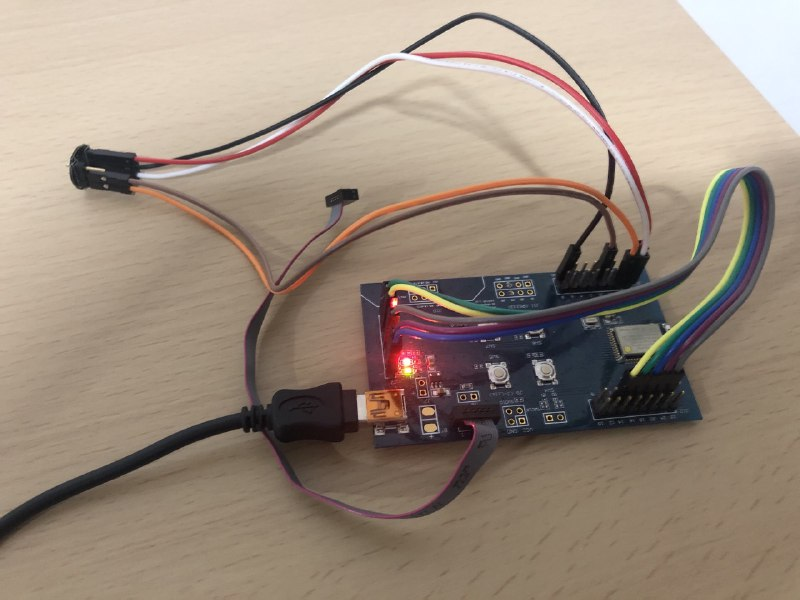
\includegraphics[scale=0.45]{./Figures/callCtrue.jpeg}	
	\caption{Llamador durante llamada en curso}
	\label{fig:Pmicon}
\end{figure}

\begin{figure}[htpb]
	\centering
   	\begin{subfigure}[b]{1\textwidth}
   		\centering
      	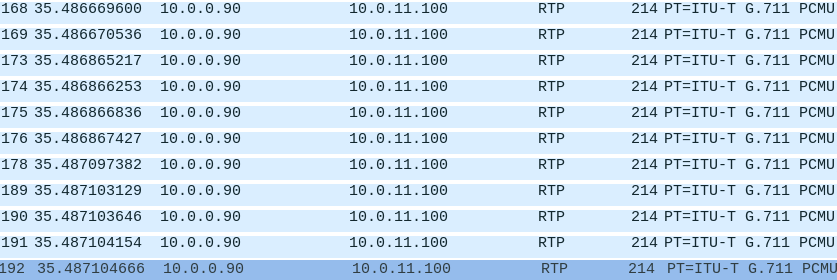
\includegraphics[width=1\textwidth]{rtp.png}
      	\caption{Paquetes RTP enviados por el terminal de sala}
      	\label{fig:PsrtpA}
   	\end{subfigure}%
   	\newline
   	\begin{subfigure}[b]{1\textwidth}
   		\centering
      	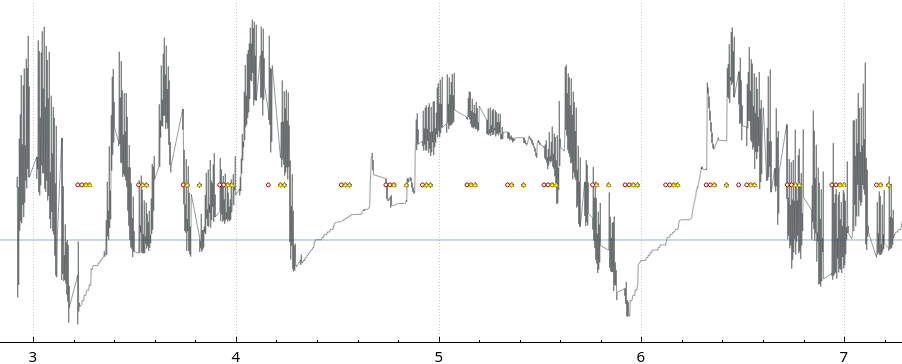
\includegraphics[width=1\textwidth]{rtpStream.png}
      	\caption{Grafica paquetes RTP enviados por el terminal de sala}
      	\label{fig:PsrtpB}
   	\end{subfigure}%
	\caption{Señal de voz enviada durante llamada}
	\label{fig:Psrtp}
\end{figure}

\section{Resultados del trabajo}
\label{sec:resTrab}

En coordinación con SURIX se realizó una demostración del funcionamiento del sistema a los ejecutivos, al personal de las áreas de ingeniería y producción de la empresa. Como conclusión de dicha demostración podemos afirmar que los resultados obtenidos fueron satisfactorios, ya que tanto los ejecutivos como el personal de la empresa manifestaron su satisfacción y beneplácito con el producto.

En otro contexto, para evidenciar las mejoras del sistema respecto al anterior, en la tabla \ref{tab:sistemasDeLLamadoEnfermera2} se compara las características de este nuevo sistema de la empresa SURIX con los productos existentes en el mercado, mencionados en el apartado \ref{sec:AntyCont}. 

\begin{table}[h]
	\centering
	\caption[Sistemas de llamado a enfermera]{Tabla comparativa de los sistemas de llamado a enfermera disponibles en el mercado}
	\begin{tabular}{l c c c c}    
		\toprule
		\textbf{Característica} 	 & \textbf{SURIX} & \textbf{MMCALL} & \textbf{Helpnex} & \textbf{SEI}\\
		\midrule
		Dispositivo llamador inalámbrico                                                    & X &   &   & X \\
Central de enfermera inalámbrica                                                    & X & X & X & X \\
\begin{tabular}[c]{@{}l@{}}Aviso de presencia de \\ enfermera por RFID\end{tabular} & X &   & X &   \\
Sistema de localización de pacientes                                                &   &   & X &   \\
Panel de control                                                                    & X & X & X & X \\
Alarma de pasillo configurable                                                      & X & X & X &   \\
Emisión de informes                                                                 & X & X & X &   \\
		\bottomrule
		\hline
	\end{tabular}
	\label{tab:sistemasDeLLamadoEnfermera2}
\end{table}
 
% Chapter Template

\chapter{Conclusiones} % Main chapter title

\label{Chapter5} % Change X to a consecutive number; for referencing this chapter elsewhere, use \ref{ChapterX}

En este capítulo se mencionan los aspectos más importantes del trabajo realizado y se contemplan los próximos pasos a seguir en el desarrollo.


%----------------------------------------------------------------------------------------

%----------------------------------------------------------------------------------------
%	SECTION 1
%----------------------------------------------------------------------------------------

\section{Conclusiones generales }

En este trabajo se implementó de manera exitosa un sistema de llamado a enfermera, inalámbrico, con conectividad bluetooth LE. Para ello se diseñaron e implementaron diferentes módulos de firmware, que permiten que un paciente solicite atención de enfermería, pudiendo incluso establecer una comunicación de voz con la enfermera asignada, todo ello a través del llamador inalámbrico que tiene asignado.

El dotar de una conectividad Bluetooth a la central de sala, la hace más versátil y abre un abanico de ampliar sus capacidades y aplicaciones no solo en el ámbito hospitalario, sino en otros ámbitos en los que SURIX trabaja.

Lastimosamente no se pudieron realizar pruebas sobre el producto final de hardware diseñado, ya que las placas electrónicas se han mandado a fabricar a China y debido a la pandemia de COVID-19, aunque se encuentran ya fabricadas está pendiente su transporte a Argentina.
Para el desarrollo del trabajo, fueron indispensables los conocimientos adquiridos en diferentes materias de la Carrera de Especialización en Sistemas Embebidos, entre las que se destacan las siguientes:


\begin{itemize}

\item Sistemas operativos de tiempo real I y II: constituyeron el primer contacto con un RTOS y permitieron aprender acerca del uso de tareas, recursos de sincronización y comunicación entre ellas, y uso de memoria e interrupciones en el contexto de un RTOS, mismos que fueron requeridos para integrar el firmware de control en el sistema de la empresa.

\item Protocolos de comunicación en sistemas embebidos: la interfaces de comunicación vistas (Bluetooth y UART) fueron una parte integral del trabajo realizado.

\item Ingeniería de software en sistemas embebidos: permitió adquirir buenas prácticas de desarrollo de software, y elaborar el diseño de algunos módulos de firmware en una etapa temprana del trabajo.

\item Desarrollo de aplicaciones en sistemas operativos de propósito general: pues se requirió desarrollar software complementario que fue de mucha ayuda al momento de validar el funcionamiento del servicio de audio desarrollado.

\end{itemize}


%----------------------------------------------------------------------------------------
%	SECTION 2
%----------------------------------------------------------------------------------------
\section{Próximos pasos}

El próximo paso lógico para el trabajo realizado será realizar las pruebas finales con el hardware de SURIX. Con el hardware probado se podrá agregar más valor al sistema con la posibilidad de agregar más servicios al dispositivo llamador, como por ejemplo un servicio que posibilite su uso para localización de pacientes dentro del hospital, característica con la que cuentan algunos sistemas del mercado.

Además, SURIX en el firmware de su terminal de sala cuenta con la posibilidad de que el software pueda ser actualizado a través de su web. Sería deseable implementar un bootloader que permita actualizar el software a través de Bluetooth, tanto de los dispositivos llamadores, como las centrales receptoras Bluetooth desarrolladas en el trabajo.

 

%----------------------------------------------------------------------------------------
%	CONTENIDO DE LA MEMORIA  - APÉNDICES
%----------------------------------------------------------------------------------------

\appendix % indicativo para indicarle a LaTeX los siguientes "capítulos" son apéndices

% Incluir los apéndices de la memoria como archivos separadas desde la carpeta Appendices
% Descomentar las líneas a medida que se escriben los apéndices

%\include{Appendices/AppendixA}
%\include{Appendices/AppendixB}
%\include{Appendices/AppendixC}

%----------------------------------------------------------------------------------------
%	BIBLIOGRAPHY
%----------------------------------------------------------------------------------------

\Urlmuskip=0mu plus 1mu\relax
\raggedright
\printbibliography[heading=bibintoc]

%----------------------------------------------------------------------------------------

\end{document}  
